\documentclass[12pt,twoside]{article}
\usepackage{chadstyle}  % Loads my formatting 
\usepackage{longtable,booktabs}
\usepackage{stmaryrd}
%%%%%%%%\usepackage{mdframed}
\usepackage{titlesec}
%\usepackage{hyperref}
%\usepackage[colorlinks,allcolors=blue]{hyperref}
%%%%%%%%%\usepackage{amsthm}
\usepackage{bbm}
\usepackage{ftnxtra}
\usepackage{fnpos}
\usepackage{multirow}
\usepackage{fontawesome}


\usepackage{bigints}
%%%%\usepackage[lite]{mtpro2}
\usepackage{physics}
\usepackage{scalerel}
\usepackage{mathrsfs}
\usepackage{empheq}

\usepackage{extarrows}
\usepackage{oubraces}
\usepackage{bm} % bold greak letters

%for algo
\usepackage{algorithm,algorithmic}
%\usepackage[noend]{algpseudocode}
%\algrenewcommand\algorithmicindent{0.5em}%


\usepackage{lmodern}
  \usepackage[T1]{fontenc}
  \usepackage[utf8]{inputenc}
  \usepackage{textcomp} % provides euro and other symbols
% use upquote if available, for straight quotes in verbatim environments
\IfFileExists{upquote.sty}{\usepackage{upquote}}{}
\usepackage{csquotes}

%\usepackage{tweaklist}  % I use this package as well; you may need to download

%% Shortcut commands

\usepackage[svgnames]{xcolor}%

\definecolor{maroon}{cmyk}{0, 0.87, 0.68, 0.32}
\definecolor{halfgray}{gray}{0.55}
\definecolor{ipython_frame}{RGB}{207, 207, 207}
\definecolor{ipython_bg}{RGB}{247, 247, 247}
\definecolor{ipython_red}{RGB}{186, 33, 33}
\definecolor{ipython_green}{RGB}{0, 128, 0}
\definecolor{ipython_cyan}{RGB}{64, 128, 128}
\definecolor{ipython_purple}{RGB}{170, 34, 255}


\usepackage[amsmath]{ntheorem}
\usepackage[ntheorem]{mdframed}
\newmdtheoremenv[linewidth=5pt, linecolor=Gainsboro!75!Lavender, topline=false, bottomline=false, skipabove=15pt, skipbelow=20pt]{thm}{\color{ChadBlue}Théorème}

\newmdtheoremenv[linewidth=5pt, linecolor=Gainsboro!75!Lavender, topline=false, bottomline=false, skipabove=15pt, skipbelow=20pt]{lemme}{\color{ChadBlue}Lemme}

\newmdtheoremenv[linewidth=5pt, linecolor=Gainsboro!75!Lavender, topline=false, bottomline=false, skipabove=15pt, skipbelow=20pt]{definition}{\color{ChadBlue}Définition}


%   \theoremclass{Theorem}
%\newtheorem{proposition}{\color{ChadBlue} Théorème}
%\newtheorem{lemme}{\color{ChadBlue} Lemme}
%\newtheorem{definition}{\color{ChadBlue} Définition}

\newcommand{\Proof}[2]{{\hspace{-\parindent} {\color{ChadBlue}\bf Démonstration}~\ref{#1}.}
{#2}\hfill$\blacksquare$ \\ \vspace{.1in}}

\newcommand{\Av}[1] {\underset {#1} {\rm Ave}\,}

\newcommand{\sinc}{\mathrm{sinc}}
\newcommand{\nn}{\nonumber}
%\newcosecnumdepthmmand{\proptitle}[1]{\color{ChadBlue} \textnormal{(#1):}}
%\newtheorem{proposition}{\color{ChadGreen} Proposition}
%\newcommand{\assume}[2]{{\bf{Assumption #1}} (#2)} 
%\newcommand{\clr}[1]{{\color{ChadBlue} #1}}
%\newcommand{\clrg}[1]{{\color{ChadGreen} #1}}
%\newcommand{\Proof}[2]{\newline {\hspace{-\parindent} {\color{ChadGreen}\bf Proof of Proposition}~\ref{#1}.}
%{\color{ChadBlue} #2} \vspace{.1in}}

% If you've loaded *tweaklist.sty* above, uncomment these lines:
% Adjust spacing in itemize/enumerate; see tweaklist.sty
%\renewcommand{\enumhook}{\setlength{\topsep}{2pt}%
%  \setlength{\itemsep}{0pt}}
%\renewcommand{\itemhook}{\setlength{\topsep}{2pt}%
%  \setlength{\itemsep}{0pt}}

\ifnum 0\ifxetex 1\fi\ifluatex 1\fi=0 % if pdftex
  \usepackage[shorthands=off,main=french]{babel}
\else
    % See issue https://github.com/reutenauer/polyglossia/issues/127
  \renewcommand*\familydefault{\sfdefault}
    % load polyglossia as late as possible as it *could* call bidi if RTL lang (e.g. Hebrew or Arabic)
  \usepackage{polyglossia}
  \setmainlanguage[]{french}
\fi

\providecommand{\tightlist}{%
  \setlength{\itemsep}{0pt}\setlength{\parskip}{0pt}}

\setcounter{secnumdepth}{4}
\setcounter{tocdepth}{3}

\titleformat{\paragraph}
{\normalfont\normalsize\bfseries}{\theparagraph}{1em}{}
\titlespacing*{\paragraph}
{0pt}{0pt}{0pt}
%{0pt}{3.25ex plus 1ex minus .2ex}{1.5ex plus .2ex}

\usepackage{setspace}
\setstretch{1.2}

%eviter les lignes blanches
\raggedbottom

\newcommand*\widefbox[1]{\fbox{\hspace{2em}#1\hspace{2em}}}
%\newcommand*\widefbox[1]{{\setlength\fboxsep{10pt}\fbox{\hspace{0.5em}#1\hspace{0.5em}}}}


\newcommand{\sklearn}{\texttt{scikit-learn}}
\newcommand{\itemb}{\item[$\bullet$]}

%JEC
\DeclarePairedDelimiter\floor{\lfloor}{\rfloor}
\DeclarePairedDelimiterX{\Iintv}[1]{\llbracket}{\rrbracket}{\iintvargs{#1}}
\NewDocumentCommand{\iintvargs}{>{\SplitArgument{1}{,}}m}
{\iintvargsaux#1} %
\NewDocumentCommand{\iintvargsaux}{mm} {#1\mkern1.5mu..\mkern1.5mu#2}


\newcommand{\fcc}[1]{\widehat{#1}^{\raisebox{1pt}{\,\scriptsize$\ast$}}}
\usepackage{stackengine}
\stackMath
\def\hatgap{2pt}
\def\subdown{-2pt}
\newcommand\reallywidehat[2][]{%
\renewcommand\stackalignment{l}%
\stackon[\hatgap]{#2}{%
\stretchto{%
    \scalerel*[\widthof{$#2$}]{\kern-.6pt\bigwedge\kern-.6pt}%
    {\rule[-\textheight/2]{1ex}{\textheight}}%WIDTH-LIMITED BIG WEDGE
}{0.5ex}% THIS SQUEEZES THE WEDGE TO 0.5ex HEIGHT
_{\smash{\belowbaseline[\subdown]{\scriptstyle#1}}}%
}}

\newcommand{\nblink}[1]{\href{https://github.com/jecampagne/ML-toys/blob/main/#1.ipynb}{\faFileCodeO}}


\usepackage{indentfirst}
%\setlength{\parindent}{1.5cm}

\usepackage{listings}


\lstset{
    breaklines=true,
    %
    extendedchars=true,
    literate=
    {á}{{\'a}}1 {é}{{\'e}}1 {í}{{\'i}}1 {ó}{{\'o}}1 {ú}{{\'u}}1
    {Á}{{\'A}}1 {É}{{\'E}}1 {Í}{{\'I}}1 {Ó}{{\'O}}1 {Ú}{{\'U}}1
    {à}{{\`a}}1 {è}{{\`e}}1 {ì}{{\`i}}1 {ò}{{\`o}}1 {ù}{{\`u}}1
    {À}{{\`A}}1 {È}{{\'E}}1 {Ì}{{\`I}}1 {Ò}{{\`O}}1 {Ù}{{\`U}}1
    {ä}{{\"a}}1 {ë}{{\"e}}1 {ï}{{\"i}}1 {ö}{{\"o}}1 {ü}{{\"u}}1
    {Ä}{{\"A}}1 {Ë}{{\"E}}1 {Ï}{{\"I}}1 {Ö}{{\"O}}1 {Ü}{{\"U}}1
    {â}{{\^a}}1 {ê}{{\^e}}1 {î}{{\^i}}1 {ô}{{\^o}}1 {û}{{\^u}}1
    {Â}{{\^A}}1 {Ê}{{\^E}}1 {Î}{{\^I}}1 {Ô}{{\^O}}1 {Û}{{\^U}}1
    {œ}{{\oe}}1 {Œ}{{\OE}}1 {æ}{{\ae}}1 {Æ}{{\AE}}1 {ß}{{\ss}}1
    {ç}{{\c c}}1 {Ç}{{\c C}}1 {ø}{{\o}}1 {å}{{\r a}}1 {Å}{{\r A}}1
    {€}{{\EUR}}1 {£}{{\pounds}}1
}

\lstdefinelanguage{iPython}{
    morekeywords={access,and,break,class,continue,def,del,elif,else,except,exec,finally,for,from,global,if,import,in,is,lambda,not,or,pass,print,raise,return,try,while},%
    %
    % Built-ins
    morekeywords=[2]{abs,all,any,basestring,bin,bool,bytearray,callable,chr,classmethod,cmp,compile,complex,delattr,dict,dir,divmod,enumerate,eval,execfile,file,filter,float,format,frozenset,getattr,globals,hasattr,hash,help,hex,id,input,int,isinstance,issubclass,iter,len,list,locals,long,map,max,memoryview,min,next,object,oct,open,ord,pow,property,range,raw_input,reduce,reload,repr,reversed,round,set,setattr,slice,sorted,staticmethod,str,sum,super,tuple,type,unichr,unicode,vars,xrange,zip,apply,buffer,coerce,intern},%
    %
    sensitive=true,%
    morecomment=[l]\#,%
    morestring=[b]',%
    morestring=[b]",%
    %
    morestring=[s]{'''}{'''},% used for documentation text (mulitiline strings)
    morestring=[s]{"""}{"""},% added by Philipp Matthias Hahn
    %
    morestring=[s]{r'}{'},% `raw' strings
    morestring=[s]{r"}{"},%
    morestring=[s]{r'''}{'''},%
    morestring=[s]{r"""}{"""},%
    morestring=[s]{u'}{'},% unicode strings
    morestring=[s]{u"}{"},%
    morestring=[s]{u'''}{'''},%
    morestring=[s]{u"""}{"""},%
    %
    % {replace}{replacement}{lenght of replace}
    % *{-}{-}{1} will not replace in comments and so on
    literate=
    {á}{{\'a}}1 {é}{{\'e}}1 {í}{{\'i}}1 {ó}{{\'o}}1 {ú}{{\'u}}1
    {Á}{{\'A}}1 {É}{{\'E}}1 {Í}{{\'I}}1 {Ó}{{\'O}}1 {Ú}{{\'U}}1
    {à}{{\`a}}1 {è}{{\`e}}1 {ì}{{\`i}}1 {ò}{{\`o}}1 {ù}{{\`u}}1
    {À}{{\`A}}1 {È}{{\'E}}1 {Ì}{{\`I}}1 {Ò}{{\`O}}1 {Ù}{{\`U}}1
    {ä}{{\"a}}1 {ë}{{\"e}}1 {ï}{{\"i}}1 {ö}{{\"o}}1 {ü}{{\"u}}1
    {Ä}{{\"A}}1 {Ë}{{\"E}}1 {Ï}{{\"I}}1 {Ö}{{\"O}}1 {Ü}{{\"U}}1
    {â}{{\^a}}1 {ê}{{\^e}}1 {î}{{\^i}}1 {ô}{{\^o}}1 {û}{{\^u}}1
    {Â}{{\^A}}1 {Ê}{{\^E}}1 {Î}{{\^I}}1 {Ô}{{\^O}}1 {Û}{{\^U}}1
    {œ}{{\oe}}1 {Œ}{{\OE}}1 {æ}{{\ae}}1 {Æ}{{\AE}}1 {ß}{{\ss}}1
    {ç}{{\c c}}1 {Ç}{{\c C}}1 {ø}{{\o}}1 {å}{{\r a}}1 {Å}{{\r A}}1
    {€}{{\EUR}}1 {£}{{\pounds}}1
    %
    {^}{{{\color{ipython_purple}\^{}}}}1
    {=}{{{\color{ipython_purple}=}}}1
    %
    {+}{{{\color{ipython_purple}+}}}1
    {-}{{{\color{ipython_purple}-}}}1
    {*}{{{\color{ipython_purple}$^\ast$}}}1
    {/}{{{\color{ipython_purple}/}}}1
    %
    {+=}{{{+=}}}1
    {-=}{{{-=}}}1
    {*=}{{{$^\ast$=}}}1
    {/=}{{{/=}}}1,
    literate=
    *{-}{{{\color{ipython_purple}-}}}1
     {?}{{{\color{ipython_purple}?}}}1,
    %
    identifierstyle=\color{black}\ttfamily,
    commentstyle=\color{ipython_cyan}\ttfamily,
    stringstyle=\color{ipython_red}\ttfamily,
    keepspaces=true,
    showspaces=false,
    showstringspaces=false,
    %
    rulecolor=\color{ipython_frame},
    frameround={t}{t}{t}{t},
    numbers=none,
    numberstyle=\tiny\color{halfgray},
    %
    %
    backgroundcolor=\color{ipython_bg},
    %   extendedchars=true,
    %basicstyle=\scriptsize,
    basicstyle=\ttfamily\footnotesize,
    columns=fullflexible,
    keywordstyle=\color{ipython_green}\ttfamily,
}

%%%%%%%%%%%%%%%%%%%%%%%%%%%%%%%%%%%%%%%%%%%%%%%%%%%%%%%%%%%%%%%%%%%%%%
%
%%%%%%%%%%%%%%%%%%%%%%%%%%%%%%%%%%%%%%%%%%%%%%%%%%%%%%%%%%%%%%%%%%%%%
\usepackage{graphicx} % Required for inserting images
\graphicspath{{figures/}}


\title{Statistiques sur générations WCRG et comparaisons avec d'autres modèles}
\author{Jean-Eric Campagne, Etienne Lempereur}
\date{\today}

\begin{document}

\maketitle
\renewcommand{\baselinestretch}{0.75}\normalsize
\tableofcontents
\renewcommand{\baselinestretch}{1.0}\normalsize

\section{Introduction}
Dans cette note est exposé une série de statistiques calculées sur des images générées par WCRG \citep{2023arXiv230600181G} en les comparant aux mêmes statistiques calculées non seulement avec les images ayant servies au training du modèle, mais aussi pour un jeu de données avec d'autres modèles comme un DGAN et un modèle micro-locale.

Brièvement, les données utilisées sont les suivantes: 
\begin{itemize}
\item[WL-1]: la motivation première était de comparer les images de Weak Lensing\footnote{La référence utilise des résultats de la simulation N-corps GadGet2.} issues d'un modèle Deep GAN de la référence \citep{2019ComAC...6....1M} avec un modèle WCRG entrainé à partir des mêmes données d'entraînement que le réseau génératif. Donc, pour le training les auteurs nous ont fourni 100,000 images 128x128 pixels, ainsi qu'un lot d'images générées par leur réseau CosmoGAN. Ainsi, nous n'avons donc pas ré-entraîné un DGAN à cette occasion. Nous avons extrait 5,000 images\footnote{C'est la statistique utilisée dans la référence \citep{2023arXiv230600181G}} pour l'entraînement d'un modèle WCRG (noté par la suite WCRG-WL1). Nous détaillons un peu plus le traitement dans la section \ref{sec:WL1}.
\item[WL-2 \& $\phi_4$]:  A la suite, de la comparaison entre le modèle WCRG-WL1 et le DGAN, nous nous sommes interrogés sur ce que les modèles WCRG entraînés sur des données WL mentionnées dans le papier \citep{2023arXiv230600181G}. Nous avons donc repris ces images d'entraînement et synthétisées pour calculer les statistiques. Idem nous avons utilisé les images d'entraînement et synthétisées par WCRG $\phi_4$ ($\beta=\{0.5, 0.68, 0.76\}$ pour calculer les dites statistiques. Cela est détaillé dans la section \ref{sec:WL2_Phi4}
\end{itemize}

Concernant la modélisation WCRG, le code python utilisé est celui du repository \url{https://github.com/Elempereur/WCRG/} mentionné dans la publication afférente.

Les statistiques utilisées sont principalement issues du code python \textit{scattering\_transform} développé par Siho Cheng\footnote{\url{https://github.com/SihaoCheng/scattering_transform} commit Fri Jun 2 11:14:53}
et utilisé entres autres dans les articles \citep{2021arXiv211201288C, 2023arXiv230617210C}. Cela concerne, le power, le bi et le tri spectra et aussi les coefficients de corrélation $C_{00}$ et $C_{01}$. Concernant les données de WL, la statistique du comptage de pics a également été utilisée. Ces statistiques sont décrites dans la section \ref{sec-summary-stat}.

Les résultats du calcul des statistiques sur les différents lots de données sont présentés dans les sections \ref{sec-WL1-res} et  \ref{sec:WL2_Phi4}.

%
\section{Modélisation WCRG sur les données WL-1}
\label{sec:WL1}
%
\subsection{Phase d'apprentissage}
\label{sec-wcrg-WL1-learning}
%
Avant l'entraînement du modèle WCRG, un traitement des données que l'on peut qualifier de "gaussianisation" a été effectué. En effet, sur la figure \ref{fig-WL1-non-trans}, on peut remarquer que la distribution des valeurs des pixels est mono-mode et peut être transformée en distribution normale par la méthode Cox-Box suivie d'une standardisation classique\footnote{Si $x$ est la valeur d'un pixel original alors primo par l'optimisation Cox-Box on trouve $\lambda^\ast \approx -0.22$, et $x^\prime = (x^{\lambda^\ast}-1)/\lambda^\ast$ suit une loi gaussienne, puis la standardisation classique permet d'obtenir une distribution normale $x^\prime \sim \mathcal{N}(0,1)$.}. Le résultat de la transformation globale est illustré sur la figure \ref{fig-WL1-trans}. Cette transformation globale (inversible) est appliquée sur tous les lots de d'images (entraînement et génération) du DGAN.
%
\begin{figure}[h]
\centering
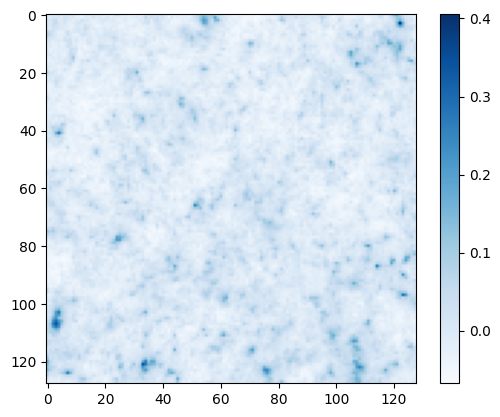
\includegraphics[width=0.4\textwidth]{fig-WL1-img-non-transformed.png}
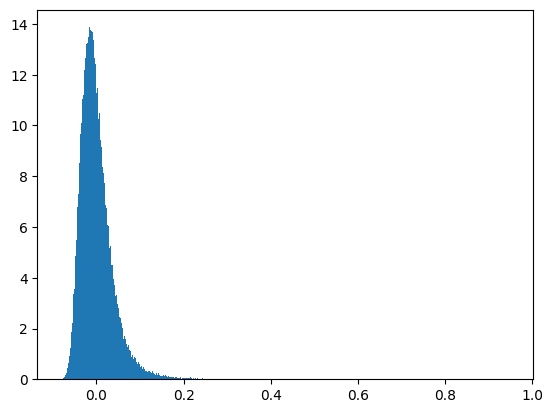
\includegraphics[width=0.45\textwidth]{fig-WL1-pixelval-non-trans.png}
\caption{Exemple d'une image du lot WL-1 (gauche) et la distribution afférente des valeurs de pixels (droite).}
\label{fig-WL1-non-trans}
\end{figure}
\begin{figure}
\centering
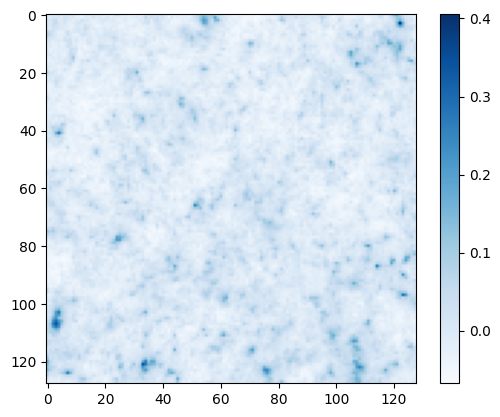
\includegraphics[width=0.45\textwidth]{fig-WL1-img-non-transformed.png}
\caption{Distribution des valeurs de pixels de la figure \ref{fig-WL1-non-trans} après application d'une transformation Cox-Box de paramètre $\lambda \approx -0.22$ et d'une standardisation classique.}
\label{fig-WL1-trans}
\end{figure}

Concernant l'optimisation du modèle WCRG\footnote{Notons que l'optimisation du modèle pourrait sans doute se passer de l'opération de gaussianisation préalable, mais l'idée était que cela pourrait aider \textit{a priori} de ne pas avoir à traiter des queues de distributions trop asymétriques.}, la démarche est très proche de celle documenté sur le repository du code, en particulier le notebook \textit{Learning\_Models.ipynb} moyennant quelques adaptations décrites ci-après.
\begin{itemize}
\itemb Les ondelettes utilisées sont de la familles Debauchies d'ordre 4 avec un padding périodique.
\itemb Pour l'ansatz $E(x_J)$ ($J=7$, $L=1$) a été utilisée la fonction 
\begin{lstlisting}[language=iPython]
def ANSATZ_NoCondi(L,centers,sigma,shifts,shifts_sym = False):
    """Non conditionnal ansatz for direct estimation of energy, a scalar potential (sigmoids) + a quadratic potential
    
    Parameters:
    L (int): system size = L*L 
    centers (tensor): position of the centers of the sigmoids 
    sigma (tensor) : width of the sigmoids
    shifts (list of tuples) : spatial shifts for the quadratic potential, carefull (0,0) is already taken into account, do not add here  
    shifts_sym (Bool) : if True, the shifts are not symetrized
    """
\end{lstlisting}
avec 20 sigmoïdes  régulièrement espacées entre le min et le max de la distribution des pixels $\approx [-100,100]$, et par ailleurs \textsf{shifts = ()}). L'optimisation SGD est menée après avoir normalisé le hessien.
%\begin{figure}[h]
%\centering
%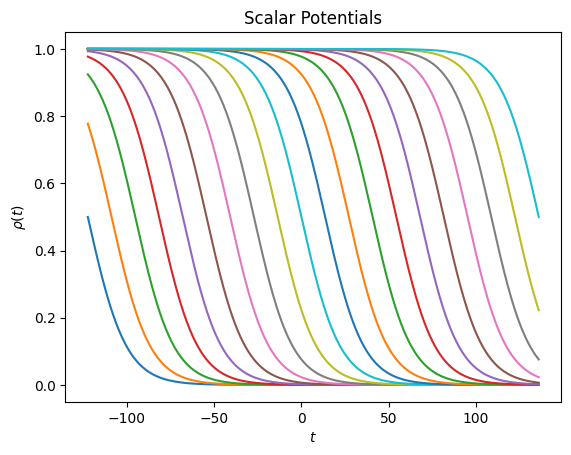
\includegraphics[width=0.4\textwidth]{fig-WL1-L1-sigmoids.png}
%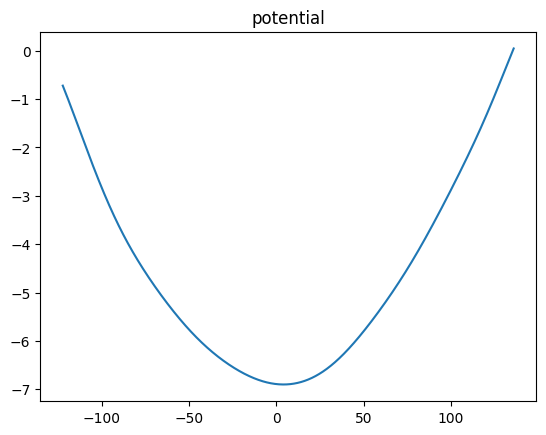
\includegraphics[width=0.4\textwidth]{fig-WL1-L1-potentiel.png}
%\caption{Scale $L=1$: sigmoïdes et potentiel optimisé.}
%\label{fig-WL1-L1}
%\end{figure}

\itemb A toutes les échelles $L>1$, nous avons utilisé la fonction 
\begin{lstlisting}[language=iPython]
def ANSATZ_Wavelet(W,L,centers,sigma,mode,shifts,shifts_sym = False):
""" Conditionnal ansatz for conditonal Energy \bar E(\bar x_j\vert x{j}) estimation with a wavelet transform,with a scalar potential (sigmoids) + a quadratic potential
    
    Parameters:
    W (Wavelet) : Wavelet to perfom fast wavelet transform
    L (int): system size ( of x_{j-1}) = L*L 
    centers (tensor): position of the centers of the sigmoids 
    sigma (tensor) : width of the sigmoids
    shifts (list of tuples) : spatial shifts for the quadratic potential, carefull (0,0) is already taken into account, do not add here 
    shifts_sym (Bool) : if True, the shifts are not symetrized
"""    
\end{lstlisting}
Tout comme pour $E_J$, l'optimisation SGD est menée après avoir normalisé le hessien.
%
\itemb A l'échelle $L=2$, 30 sigmoïdes régulièrement espacées dans l'intervalle $[-75, 75]$ sont utilisées, tandis que \textsf{extend = 1.0}. Les autres paramètres sont \textsf{mode = 'All'} et \textsf{shifts = ()}.  
%\begin{figure}[h]
%\centering
%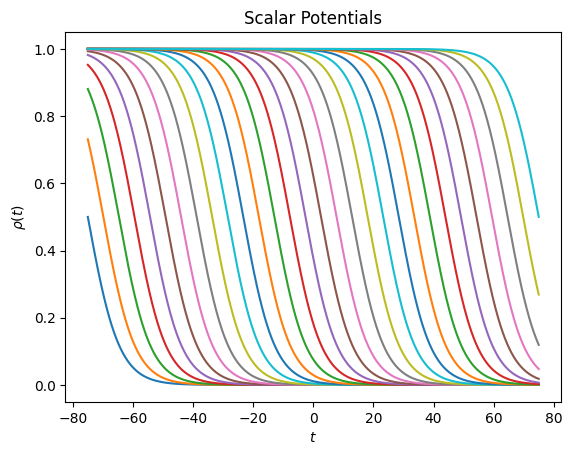
\includegraphics[width=0.4\textwidth]{fig-WL1-L2-sigmoids.png}
%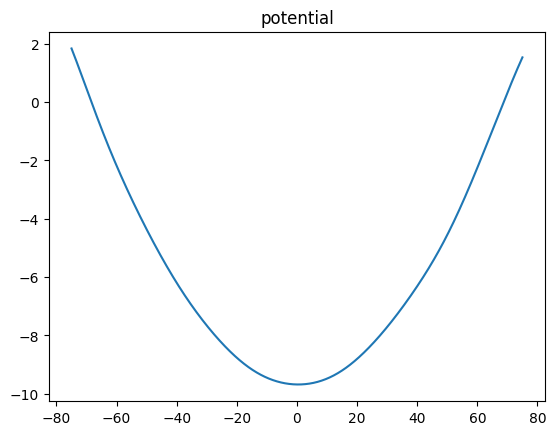
\includegraphics[width=0.4\textwidth]{fig-WL1-L2-potentiel.png}
%\caption{Scale $L=2$: même légende que la figure \ref{fig-WL1-L1}.}
%\label{fig-WL1-L2}
%\end{figure}

%
\itemb A l'échelle $L=4$,  30 sigmoïdes sont également utilisées mais cette fois réparties uniformément selon les quantiles avec $q_{min}=10^{-5}$, $q_{max}=1.0$ et \textsf{extend = 1.0}. De plus \textsf{mode = 'All'} tandis que \textsf{shifts = ((1,0),(0,1),(1,1))} conjointement à \textsf{shifts\_sym = True}.
%
\itemb A l'échelle $L=8$, on utilise 40 sigmoïdes réparties uniformément selon les quantiles avec $q_{min}=10^{-5}$, $q_{max}=1.0$ et \textsf{extend = 1.0}. Par ailleurs outre \textsf{mode = 'All'}, nous avons utilisé la fonction suivante pour définir les shifts tels que 
\textsf{shifts =shift\_modif(L//4)}.
\begin{lstlisting}[language=iPython]
def shift_modif(n):
    shifts =[]
    for i in range(-n,n):
        for j in range(-n,n):
            if i==0 and j==0:
                pass
            else:
                shifts.append((i,j))
    return shifts
\end{lstlisting}
%
\itemb A l'échelle $L=16$, se sont 40 sigmoïdes uniformément réparties sur l'intervalle $[-30, 30]$ que l'on utilise avec \textsf{extend = 1.0}. Par ailleurs \textsf{mode = 'All'} et 
\textsf{shifts =shift\_modif(L//4)}.
%
\itemb A l'échelle $L=32$, on utilise comme précédemment 40 sigmoïdes uniformément réparties sur l'intervalle $[-20, 20]$ (\textsf{extend = 1.0}). Les paramètres \textsf{extend}, \textsf{mode} et \textsf{shifts} sont les mêmes valeurs pour les deux premiers et définition pour le dernier que pour l'échelle précédente.
%
\itemb A l'échelle $L=64$, on utilise 30 sigmoïdes réparties uniformément selon les quantiles avec $q_{min}=10^{-5}$, $q_{max}=1.0$ et \textsf{extend = 1.0}. De plus si \textsf{mode = 'All'} comme précédemment, par contre \textsf{shifts = shift\_modif(L//8)}.
%
\itemb Enfin à l'échelle $L=128$ (taille des images d'entraînement), on utilise comme  30 sigmoïdes uniformément réparties sur l'intervalle $[-7.0, 5.5]$ (\textsf{extend = 0.25}), et si \textsf{mode = 'All'} comme précédemment, par contre \textsf{shifts = shift\_modif(L//16)}.
%
\itemb Les paramètres qui sont particulièrement délicats affectant la synthèse des images aux différentes échelles, sont ceux qui définissent les centres des sigmoïdes (l'intervalle $[min,max]$ pour \textsf{linspace\_centers}, ou $[q_{min},q_{max}]$ pour \textsf{quantile\_centers}. La méthode \textsf{shift\_modif} a été utilisée in fine mais ne change pas vraiment les résultats par rapport à l'usage de \textsf{shift\_quad\_Sym} utilisée de prime abord. Les optimisations SGD sont souvent reprises pour un peu tuner les paramètres tels que le nombre d'époques \textsf{num\_epochs} et le learning rate \text{lr}. Parfois deux étapes d'optimisation ont été pratiquées, notamment avec une valeur de  \text{lr} plus petite pour la seconde étape.
\end{itemize}
%

Une fois les paramètres "optimisés" (par ex. les sigmoïdes), les différents potentiels appris $\bar{v}_j(x_{j-1})$ sont présentés sur la figure \ref{fig-WL1-potentiels-optim}.

\begin{figure}
\centering
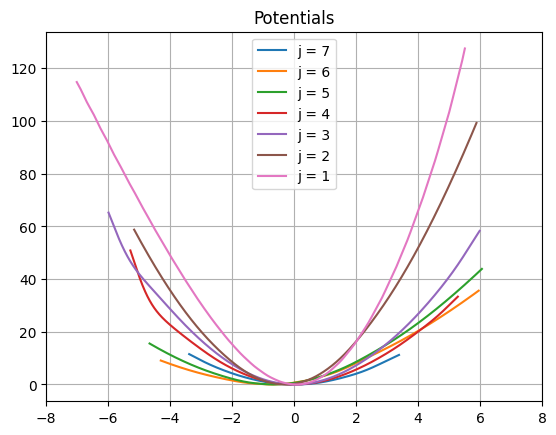
\includegraphics[width=0.8\textwidth]{fig-WL1-potentiels-optim.png}
\caption{Potentiels scalaires équivalents $\bar{v}_j$ appris à chaque échelle $j$ pour les images de WL-1.}
\label{fig-WL1-potentiels-optim}
\end{figure}
%
\subsection{Phase de synthèse}
\label{sec-wcrg-WL1-synt}
%
Une fois le modèle appris, on peut regarder à chaque échelle la qualité des synthèses. En fait, à dire vrai, les paramètres qui définissent les sigmoïdes à toutes les échelles ont été ajustés à la main largement pour que les histogrammes de contrôles montre une bonne adéquation entre images d'origines et images de synthèse. La technique de sampling est en tout point identique à celle mise en œuvre pour l'article. Ce qui peut changer concerne le nombre de steps et la taille de chaque step. \textit{Même si la suite pourrait paraître fastidieuse et répétitive, dans cette note une certaine exhaustivité s'impose néanmoins surtout que les codes n'ont pu être tournés sur notebooks partageables.} 

A l'échelle $L=1$, la comparaison des distributions de valeurs de pixels entre données d'entraînement et synthétisées est montrée sur la figure \ref{fig-WL1-synt-L1-pixelval} de l'appendix. Aux échelles suivantes, outre la comparaison des distributions des valeurs de pixels des images originales et synthétisées, on peut également questionner la distribution des cartes de détails hautes fréquences (horizontales/verticales/diagonales) obtenues par décomposition en ondelettes.
Les résultats aux échelles $L\in[1,128]$ sont présentés sur les figures de \ref{fig-WL1-synt-L2} à \ref{fig-WL1-synt-L128} de l'appendix. Pour des raisons tenant à la taille mémoire des GPUs utilisés, le nombre de cartes générées jusqu'à l'échelle 16 incluse est de 5000, tandis que pour les échelles supérieures on ne peut disposer que de 500 cartes.

A l'échelle $L=128$, on dispose de cartes synthétisées "finales" qui si tout se passe au mieux doivent ressembler comme deux gouttes d'eau aux cartes utilisées pour l'entraînement (ou cartes "originales"). La figure \ref{fig-WL1-synt-exemples} donne quelques exemples de cartes originales et synthétisées.
%
\begin{figure}
\centering
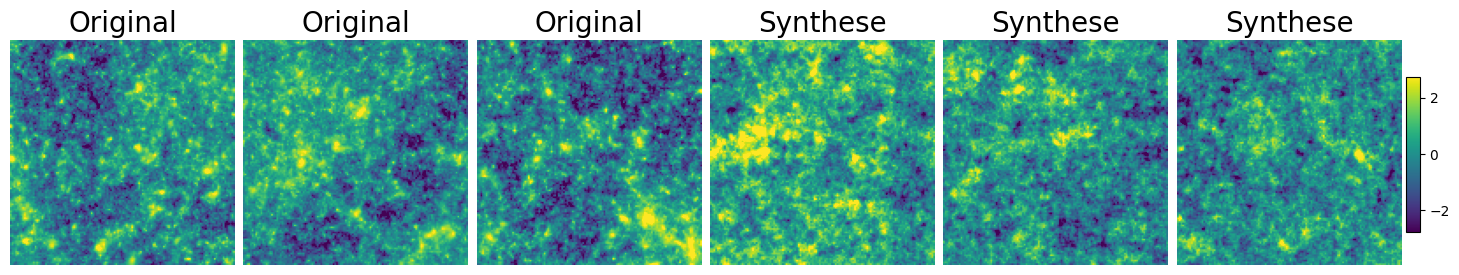
\includegraphics[width=0.99\textwidth]{fig-WL1-synt-exemples.png}
\caption{Exemples de cartes WL-1 utilisées pour l'entraînement et synthétisées une fois le modèles WCRG optimisé.}
\label{fig-WL1-synt-exemples}
\end{figure}
% 
Il est indéniable que le modèle a appris quelque chose. Maintenant, dans l'article \citep{2023arXiv230600181G}, il est montré non seulement des cartes synthétisées, la distribution des valeurs de pixels\footnote{nb. le modèle de l'article a été optimisé directement sur les cartes de WL-2 sans transformation préalable donc on ne peut comparer les modèles. Cela sera sans doute à revoir ultérieurement.} mais aussi la comparaison  du spectre de puissance. Ce dernier point a motivé l'usage de statistiques afin de caractériser les distributions des pixels et de comparer ces statistiques obtenues sur les cartes originales et les synthétisées. Ceci est présenté dans la section suivante.
%
\section{Réduction d'information par l'usage de statistiques}
\label{sec-summary-stat}
%
Un certain nombre de statistiques ont été utilisées afin d'aller au-delà de l'aspect visuel jugeant de la qualité de la synthèse des cartes de WL-1. Comme mentionné dans l'introduction, en premier lieu il a été utilisé le code développé par Siho Cheng afin de calculer:
\begin{itemize}
\itemb les classiques spectre de puissance, \textit{bi}-spectre et \textit{tri}-spectre; 
\itemb le coefficient de scattering $S1_{iso}$, ainsi que les coefficients composites $s_{21}$ (sparsity) et $s_{22}$ (shape) définis dans la référence \citep{2021arXiv211201288C}; 
\itemb mais aussi les versions \textit{isotropiques} des corrélations de scattering définies selon\footnote{$\langle x \rangle =\Av{u}(x(u))$.}
\begin{eqnarray}
 C_{01} &=& \langle(I \ast \psi_2)(|I \ast \psi_1| \ast \psi_2)^\ast\rangle / factor \\
 C_{11} &=& \langle(|I \ast \psi_1| * \psi_3)(|I * \psi_2| * \psi_3)^\ast\rangle / factor
\end{eqnarray}
avec $I$ la carte de champ, $\psi_i$ des ondelettes de Morlet à différentes échelles et orientations et où le choix de normalisation est défini par
\begin{equation}
factor = L2(I \ast \psi_1) \times L2(I \ast \psi_2)
\end{equation}
Les définitions de ces facteurs sont décrites dans l'article \citep{2023arXiv230617210C}: $C_{01}$ et $C_{11}$ correspondent respectivement à $\tilde{S}_3$ et $\tilde{S}_4$, et la version "iso" opère une réduction sur les paires d'angles. 
\end{itemize}

En pratique afin de fixer un peu les idées, l'obtention des différents spectres et coefficients  s'effectue schématiquement selon les étapes suivantes (si "maps" correspond à un lot de cartes):
\begin{lstlisting}[language=iPython]
bins_pw = 30
Nmaps,M,N = maps.shape
J = int(np.log2(min(M,N))) - 1
pw, kr  = scattering.get_power_spectrum(maps,
              k_range=np.logspace(0,np.log10(M/2*1.4), 
              bins_pw+1))
bi_calc = scattering.Bispectrum_Calculator(M,N, 
              k_range=np.logspace(0,np.log10(M/2*1.4), J-1))
tri_calc = scattering.Trispectrum_Calculator(M,N,
              k_range=np.logspace(0,np.log10(M/2*1.4), J-1))

st_calc = scattering.Scattering2d(M, N, J=6, L=4)

coeffs = st_calc.scattering_coef(maps)
s1  = np.log10(coeffs['S1_iso'])
s21 = np.log10(coeffs['s21'])
s22 = np.log10(coeffs['s22'])

cov_coef = st_calc.scattering_cov(maps)
select_and_index = get_scattering_index(J, L, normalization='P00', C11_criteria='j2>=j1')
c01 = cov_coef['C01_iso'][:,select_and_index['select_2_iso']]
c11 = cov_coef['C11_iso'][:,select_and_index['select_3_iso']]
\end{lstlisting}
De plus, afin de satisfaire des contraintes de taille de mémoire, les spectres/coefficients ont été calculés sur des lots de cartes dont on en a tiré des moyennes et écarts-types (barres d'erreur dans les histogrammes).

Dans le cas des cartes de WL, on a également utilisé le comptage de "pics" au dessus d'un seuil. Il s'agit d'une statistique d'ordre supérieur à la recherche des non-gaussianité qui s'est répandue récemment (voir la référence \cite{2023arXiv230507531L} et les références incluses). Pour se faire la méthode détaillée dans l'article de D. Lanizieri et al. a été utilisée\footnote{\url{https://github.com/LSSTDESC/DifferentiableHOS.git}} avec à la base la fonction \textsf{find\_peaks2d\_tf} du package \textsf{lenspack}\footnote{\url{https://github.com/CosmoStat/lenspack}} qui cherche la localisation des pics ainsi que leurs "hauteurs", puis un lissage par un noyau gaussien. Le résultat est donc un histogramme de la distribution smoothée des hauteurs de pics d'une carte (ou d'un lot de cartes). Un exemple de recherche de pics pour un seuil de $2$ est donné sur la figure \ref{fig-WL-peakcount-thr2-exemple}.
\begin{figure}
\centering
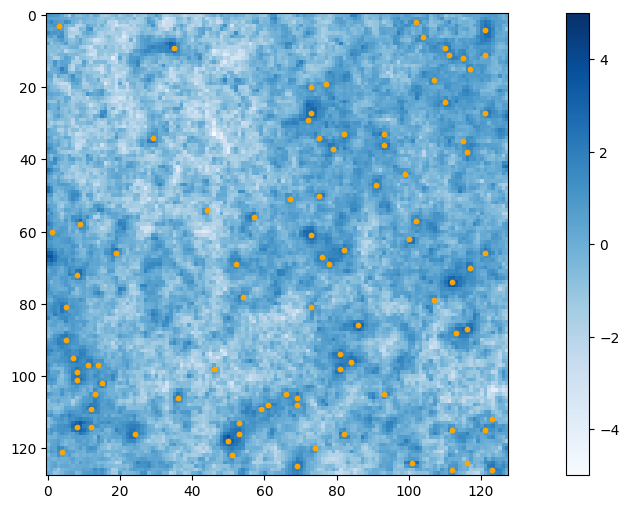
\includegraphics[width=0.4\textwidth]{fig-WL-peakcount-thr2-exemple.png}
\caption{Exemples de la recherche de pics au dessus d'un seuil ici pris à 2.}
\label{fig-WL-peakcount-thr2-exemple}
\end{figure}
%
\section{Résultats concernant les données WL-1}
\label{sec-WL1-res}
%
Une fois le modèle WCRG obtenu selon la méthode détaillée à la section \ref{sec-wcrg-WL1-learning}, on peut calculer les statistiques décrites dans la section précédente non seulement sur des cartes générées (Sec.~\ref{sec-wcrg-WL1-synt}) mais aussi sur des cartes ayant servi à l'apprentissage du modèle. Les résultats sont présentés sur la figure \ref{fig-WL1-summary-stat} sous les appellations "wcrg" (rouge) et "train" (bleu). Il est assez remarquable que la quasi totalité des distributions issues de la génération de cartes par le modèle WCRG soient bien, voire très bien reproduite. 
\begin{figure}
\centering
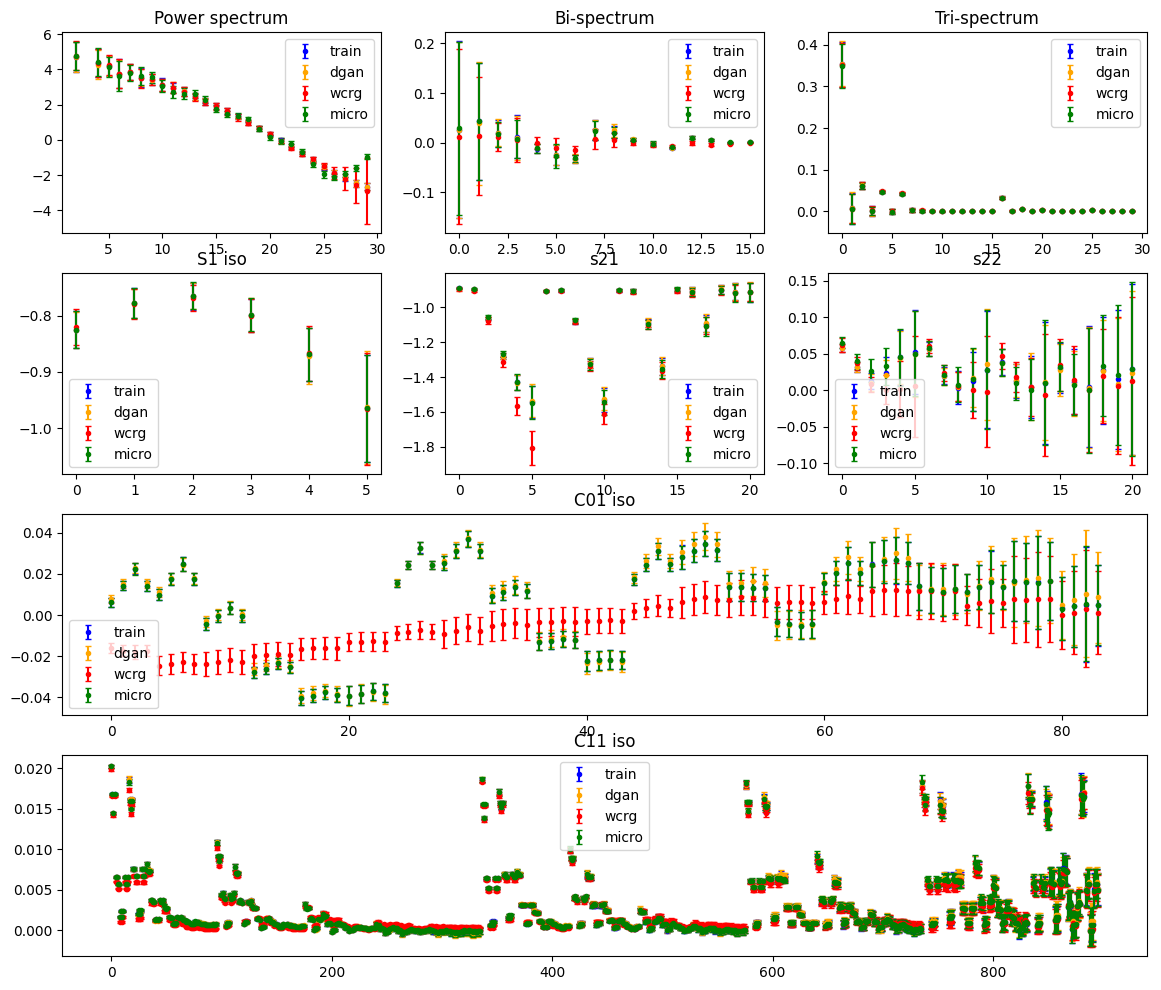
\includegraphics[width=0.99\textwidth]{fig-WL1-summary-stat.png}\\
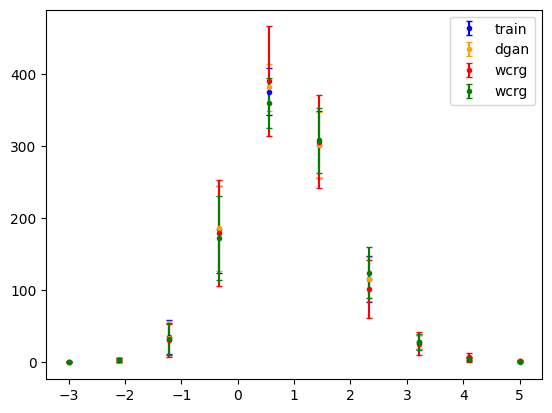
\includegraphics[width=0.4\textwidth]{fig-WL1-peak-count.png}
\caption{Histogrammes des statistiques détaillées à la section \ref{sec-summary-stat}. Il est a noté qu'excepté le comptage de pics, les distributions sont calculées avec 500 cartes.}
\label{fig-WL1-summary-stat}
\end{figure}
Donc, il n'est pas étonnant que les différences que nous pointons par la suite n'aient pas été mise en évidence dans l'article \citep{2023arXiv230600181G}.

Si on se penche sur les distributions qui dénotent, on constate que:
\begin{itemize}
\itemb en premier lieu ce qui questionne concerne la distribution $C_{01}^{iso}$ qui manifestement a un problème, alors que la distribution $C_{11}^{iso}$ est bien reproduite;
\itemb dans une moindre mesure on constate aussi que le bi-spectre ($s_{21}$) est moins bien reproduit que le tri-spectre ($s_{22}$).
\end{itemize} 
C'est deux points dont l'origine peut être la même, a motiver les investigations suivantes.

Notons que si l'on prend les cartes  issues de la génération du réseau CosmoGAN mentionné en introduction, il y a un parfait accord de toutes les distributions "dgan" (orange) avec les distribution d'entraînement ("train"). En ce sens, le GAN fait mieux sur ce critère\footnote{Rappel: à l'origine de l'étude était la comparaison "dgan", "wcrg", et dans ce contexte le nombre d'images ayant servit à l'entraînement du modère WCRG est de 5,000 images alors que le DGAN en a utilisé 200,000 \citep{2019ComAC...6....1M}}.  

Nous avons également procédé à la synthèses de cartes en utilisant une modélisation micro-canonique \citep{2023arXiv230617210C} à l'aide du code de Siho Cheng selon typiquement 
\begin{lstlisting}[language=iPython]
 st_calc.scattering_cov(...)['for_synthesis']
\end{lstlisting}
qui utilise les paramètres: le rapport $\langle I\rangle/\sigma(I)$, $L2(I\ast \psi_i)$, $S_1$, ainsi que les parties réelles et imaginaires des coefficients de corrélation $C_{01}$ et $C_{01}$
Ce type de modélisation/synthèse notée "micro"(vert) sur la Fig.~\ref{fig-WL1-summary-stat} reproduit très bien la quasi totalité des distributions exceptée\footnote{Si l'on ne porte que les distributions "train" et "micro", la remontée du spectre de puissance "micro" est bien visible.} le spectre de puissance à grande valeur de $k$ même si on note que les fluctuations des valeurs sont bien plus réduites que pour les autres modèles pourtant calculées avec le même nombre de cartes. Ceci, concernant les coefficients $C_{01}$ l'accord est parfait, mais on s'en doutait puisqu'ils rentrent dans la liste des paramètres ayant servi pour définir la métrique à minimiser afin de produire le modèle micro-canonique.

Dans les sections suivantes, nous allons utiliser les cartes générées par les modèles WCRG ainsi que celles d'entraînement de type WL-2 et $\phi_4$ décrites dans l'introduction, afin de savoir si ces modèles performent mieux ou pas.
%
\section{Modèles WCRG et données WL-2 et $\phi_4$}
\label{sec:WL2_Phi4}
%
La question qui vient est de savoir pour quelles raisons la distribution $C_{01}^{iso}$ (et aussi bi-spectre et $s_{21}$) est nettement moins bien reproduite par le modèle WCRG optimisé comme décrit à la section \ref{sec-wcrg-WL1-learning}. Pour se faire, nous avons utilisé directement (c'est-à-dire sans nouveau entraînement) les modèles et les données de l'article \citep{2023arXiv230600181G}.

Concernant les données WL-2, on dispose pour le calcul des statistiques de 500 cartes d'entraînement ("train") et de 209 cartes générées ("wcrg"). Une note technique: nous avons procéder à un recalage de la distribution des valeurs de pixels des cartes générées afin que la moyenne soit égale à celle des cartes d'entraînement, mais nous n'avons pas opéré de gaussianisation (cf. Sec.~\ref{sec-wcrg-WL1-learning}). Les résultats sont présentés sur la figure \ref{fig-WL2-summary-stat}.
\begin{figure}
\centering
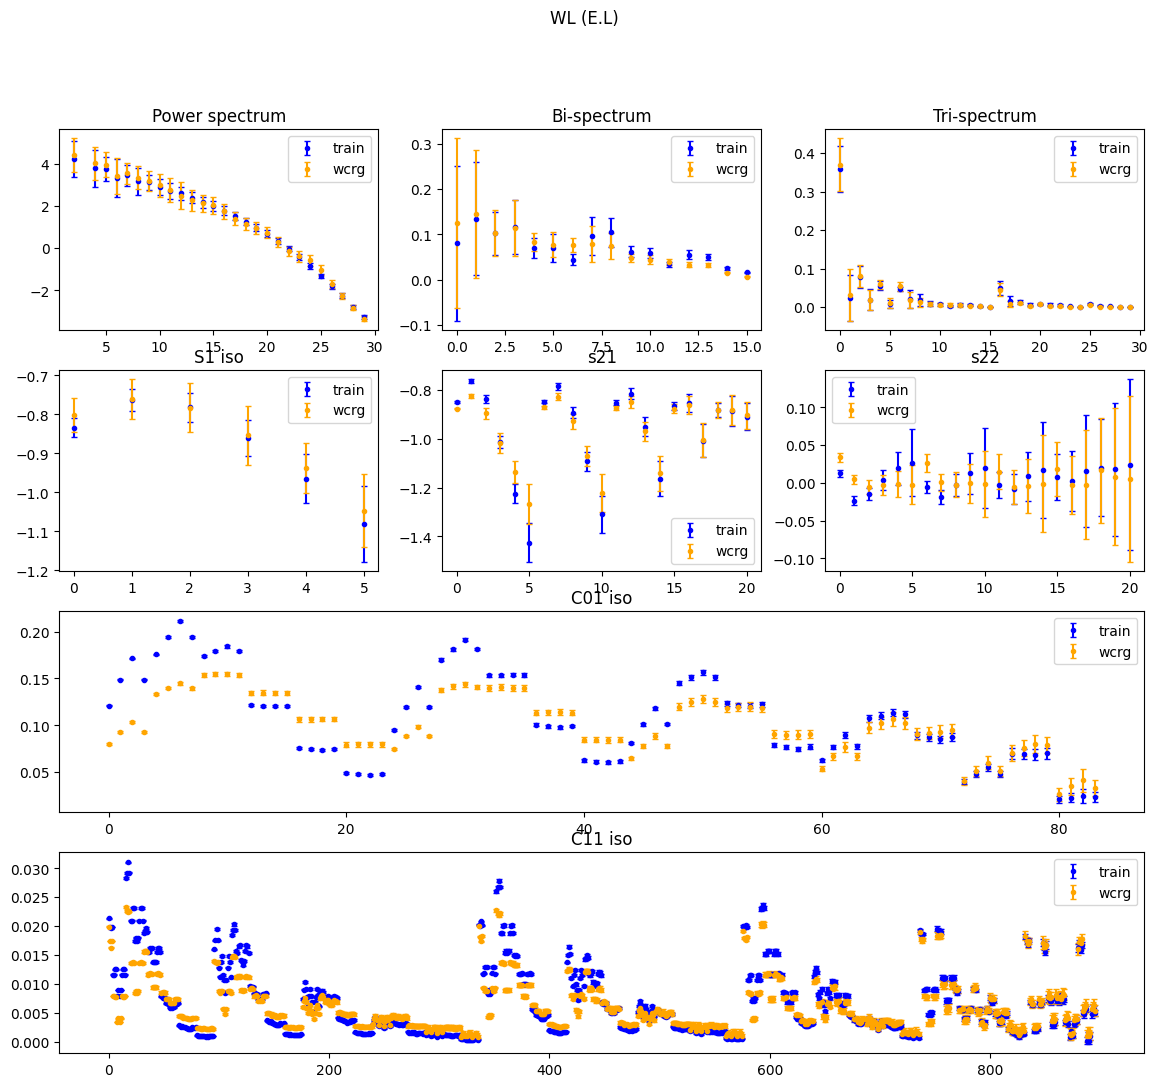
\includegraphics[width=0.99\textwidth]{fig-WL2-summary-stat.png}\\
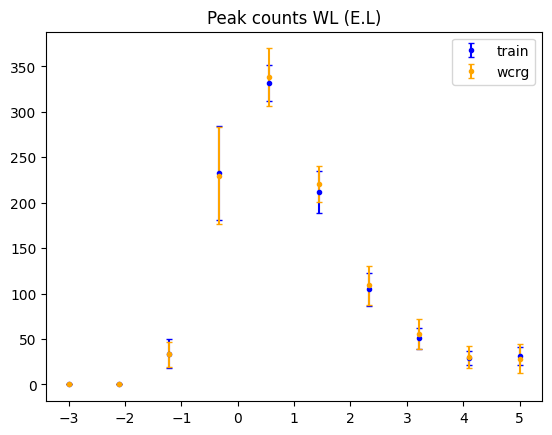
\includegraphics[width=0.4\textwidth]{fig-WL2-peak-count.png}
\caption{Statistiques de la figure \ref{fig-WL1-summary-stat} mais concernant les données WL-2.}
\label{fig-WL2-summary-stat}
\end{figure}
Par rapport à la figure \ref{fig-WL1-summary-stat} utilisant un modèle optimisé sur les données WL-1 (gaussianisée), on constate 
\begin{itemize}
\itemb primo que la distribution des $C_{01}^{iso}$  calculées avec les cartes générées ("wcrg") suit les ondulations de la distribution calculée sur les données d'entraînement ("train"). Mais il y a un petit désaccord néanmoins mais bien plus petit qu'en même.
\itemb les petits désaccords sur les distribution bi-spectre et $s_{21}$ sont de même ampleur
\itemb on note également petit désaccord  sur la distribution des $C_{11}^{iso}$.
\end{itemize}
Ce premier point nous renseigne sur le fait qu'un modèle WCRG est capable de générer des cartes avec des coefficients $C_{01}^{iso}$ convenables en tous les cas bien plus que ceux de la figure \ref{fig-WL1-summary-stat}. 

Concernant les données $\phi_4$, on dispose de 3 lots obtenus avec les valeurs de $\beta$ différentes ($\{0.5,\ 0.68,\ 0.76\}$) qui influencent la dynamique sous-jacente. Tout comme pour les cartes WL-2, on a procédé à l'accord des moyennes des distributions des valeurs de pixles entre les cartes générées et les  cartes d'entraînement. Les différents résultats sont exposés sur les figures \ref{fig-phi4-b050-summary-stat}, \ref{fig-phi4-b068-summary-stat}, et \ref{fig-phi4-b076-summary-stat}.

\begin{figure}
\centering
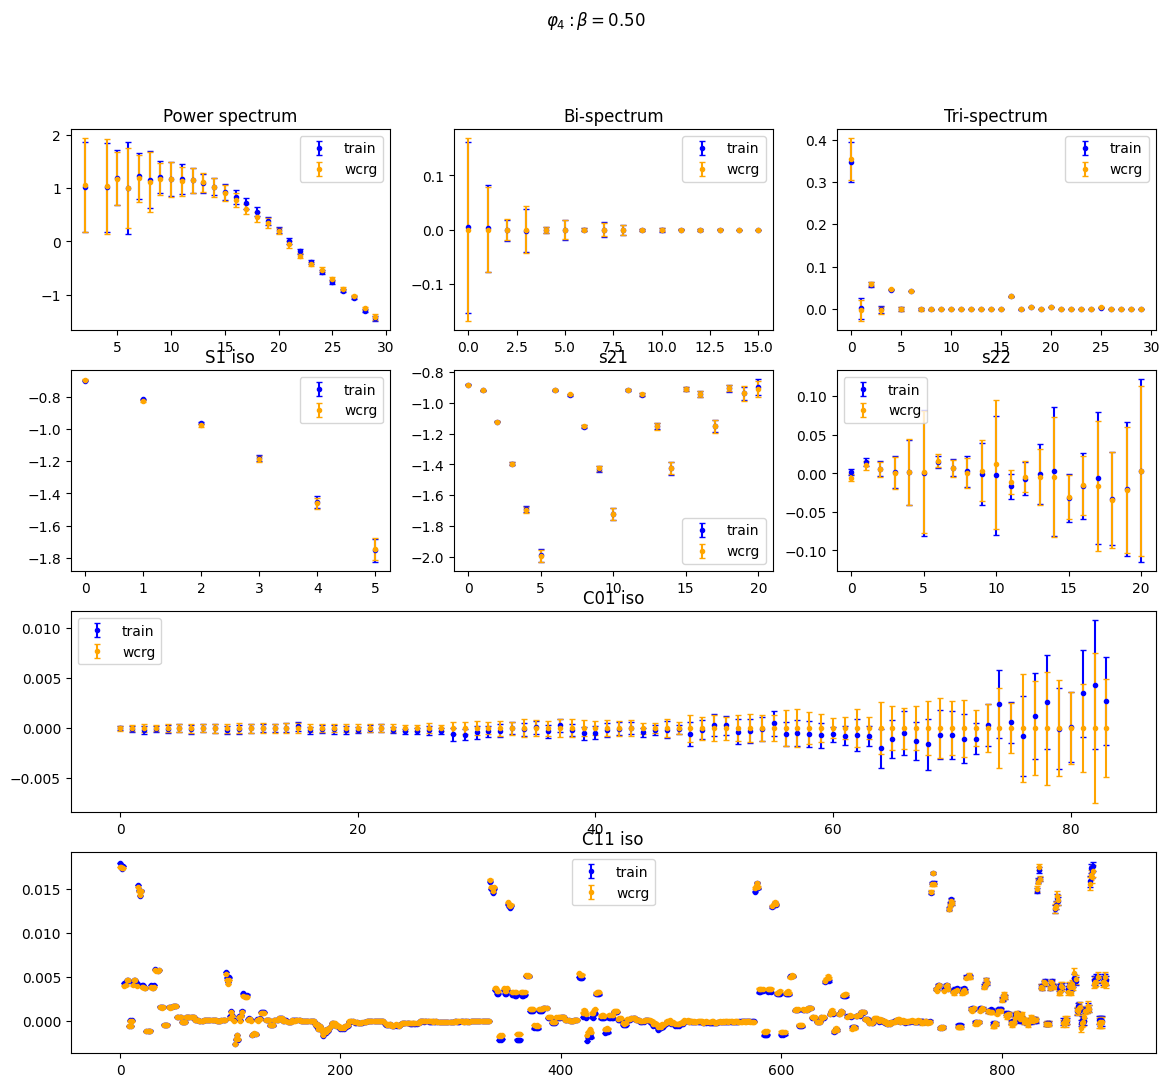
\includegraphics[width=0.99\textwidth]{fig-phi4-b050-summary-stat.png}
\caption{Statistiques de la figure \ref{fig-WL1-summary-stat} mais concernant les données $\phi_4$ ($\beta=0.50$).  Notons que l'on dispose de 500 cartes "train" et de 400 cartes "wcrg".}
\label{fig-phi4-b050-summary-stat}
\end{figure}

\begin{figure}
\centering
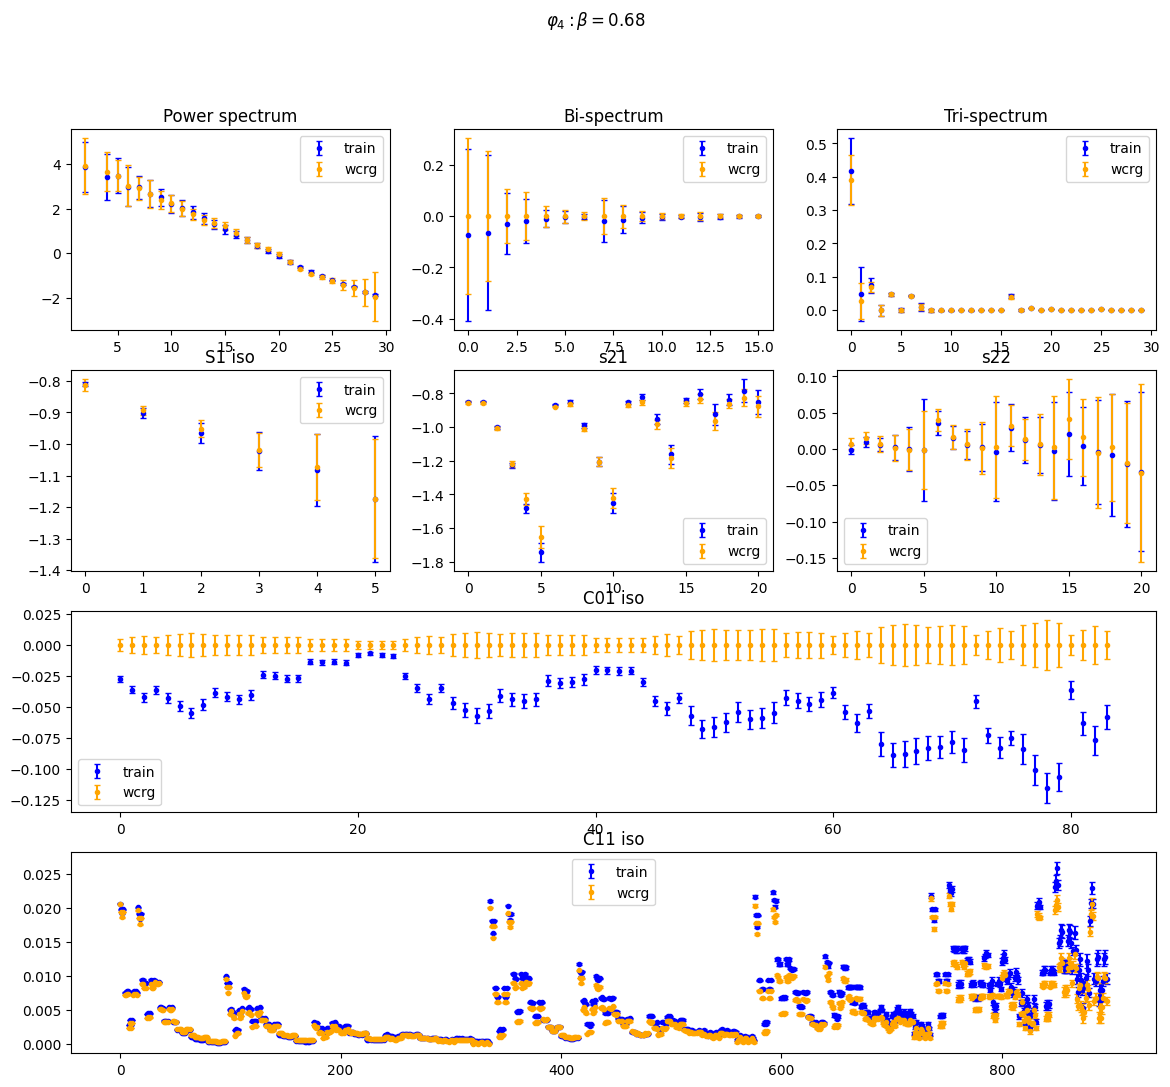
\includegraphics[width=0.99\textwidth]{fig-phi4-b068-summary-stat.png}
\caption{Statistiques de la figure \ref{fig-WL1-summary-stat} mais concernant les données $\phi_4$ ($\beta=0.68$). Notons que l'on dispose de 500 cartes "train" et de 500 cartes "wcrg".}
\label{fig-phi4-b068-summary-stat}
\end{figure}

\begin{figure}
\centering
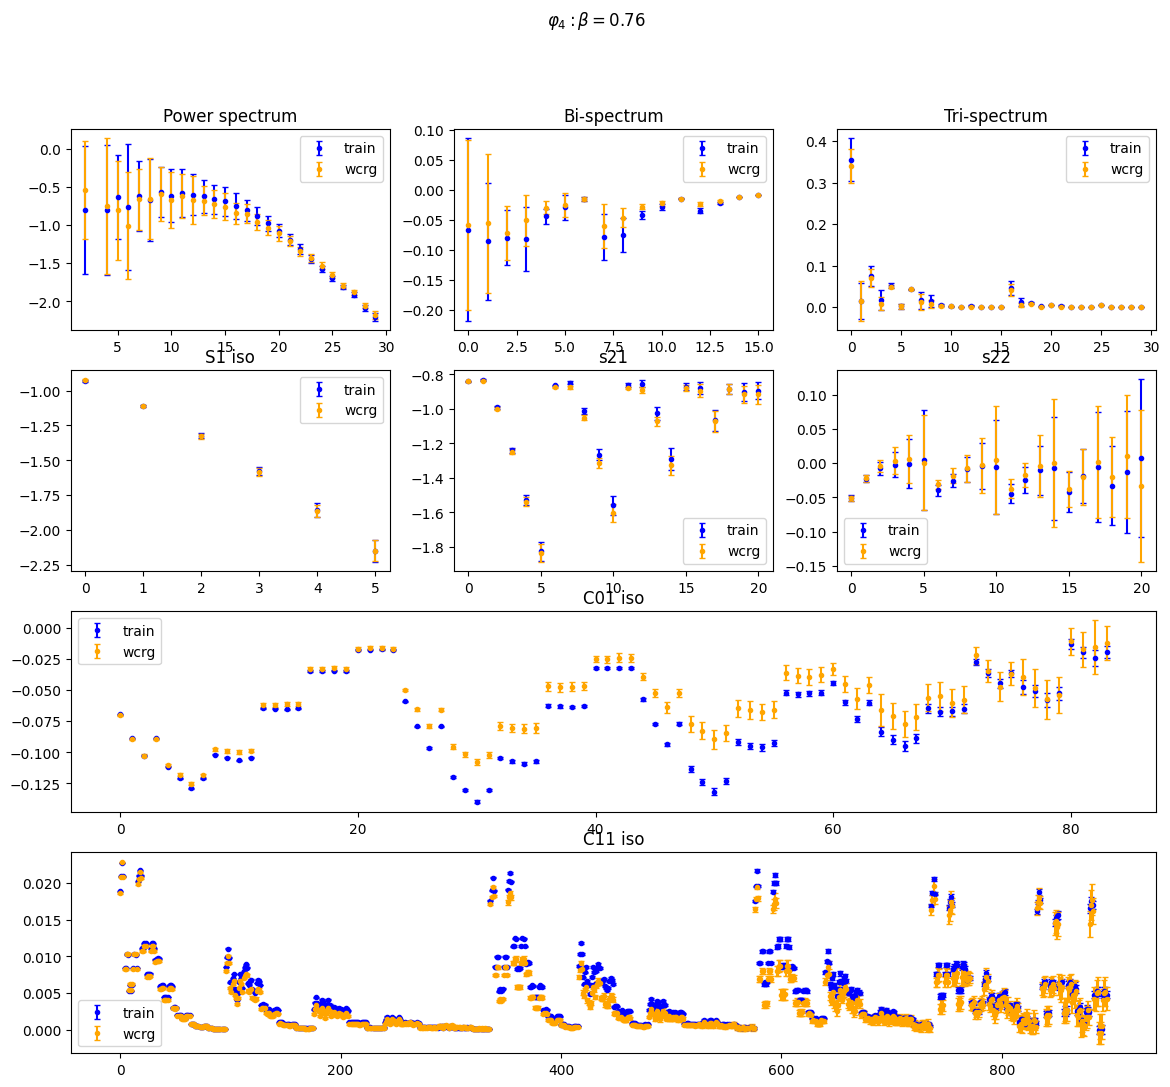
\includegraphics[width=0.99\textwidth]{fig-phi4-b076-summary-stat.png}
\caption{Statistiques de la figure \ref{fig-WL1-summary-stat} mais concernant les données $\phi_4$ ($\beta=0.76$). Notons que l'on dispose de 500 cartes "train" et de 50 cartes "wcrg".}
\label{fig-phi4-b076-summary-stat}
\end{figure}

Ce que l'on constate c'est que:
\begin{itemize}
\itemb les distributions obtenues avec les données $\beta=0.50$ sont remarquablement concordantes; et notons que les coefficients $C_{01}^{iso}$ même sur les données d'entraînement sont quasi-nuls.
\itemb les désaccords entre les distributions avec les données $\beta=0.76$ sont assez semblables à ceux observés sur les données $WL$.
\itemb la figure des distributions des coefficients $C_{01}^{iso}$ avec les données $\beta=0.76$ est particulière: les coefficients calculés avec les données générées sont quasi-nuls, or on constate une structuration de la distribution calculée avec les données d'entraînement. Notons que contrairement au cas $WL$ la distribution du bi-spectre semble bien reproduite (aux erreurs statistiques près), et il en va de même avec la distribution $s_{21}$.
\end{itemize}
Ainsi, on dispose de plusieurs cas de figures et à part 1 cas ($\phi_4$, $\beta=0.50$) tous les autres exhibent des divergences concernant principalement les coefficients $C_{01}^{iso}$. Même si on n'exclut pas un bug sous-jacent, les distributions de ces coefficients générés montrent tout de même des structures sauf précisément pour $\phi_4$, $\beta=0.50$.

Deux expérimentations ont été menées pour essayer de comprendre la distribution des $C_{01}^{iso}$:
\begin{itemize}
\itemb la première concerne les données WL-1 mais avec les cartes à l'échelle $L=64$. Le résultat est présenté sur la figure \ref{fig-WL1-64x64-summary-stat}. Les désaccords des distributions $C_{01}^{iso}$ sont présents. Notons que les autres distributions sont très bien reproduites. 
\begin{figure}
\centering
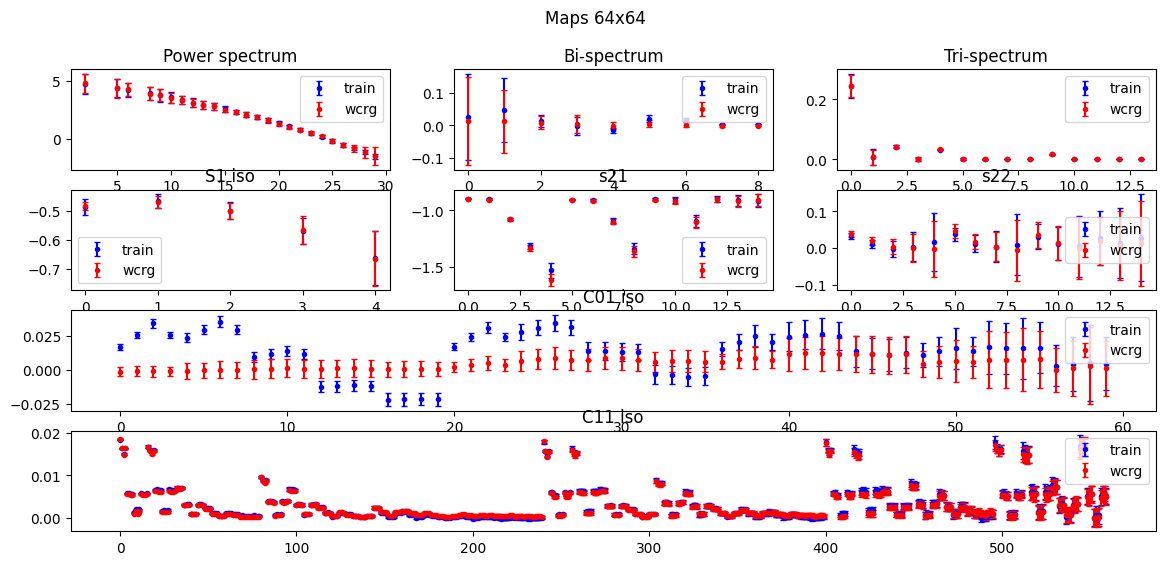
\includegraphics[width=0.99\textwidth]{fig-WL1-64x64-summary-stat.png}
\caption{Statistiques de la figure \ref{fig-WL1-summary-stat} mais concernant les données WL-1 à l'échelle $L=64$. Notons que l'on dispose de 500 cartes "train" et de 50 cartes "wcrg".}
\label{fig-WL1-64x64-summary-stat}
\end{figure}
\itemb la seconde reprend la synthèse avec un modèle micro-canonique mais où l'on a volontairement fixé à 0 les coefficients $C_{01}$. Le résultat est illustré sur la figure 
\begin{figure}
\centering
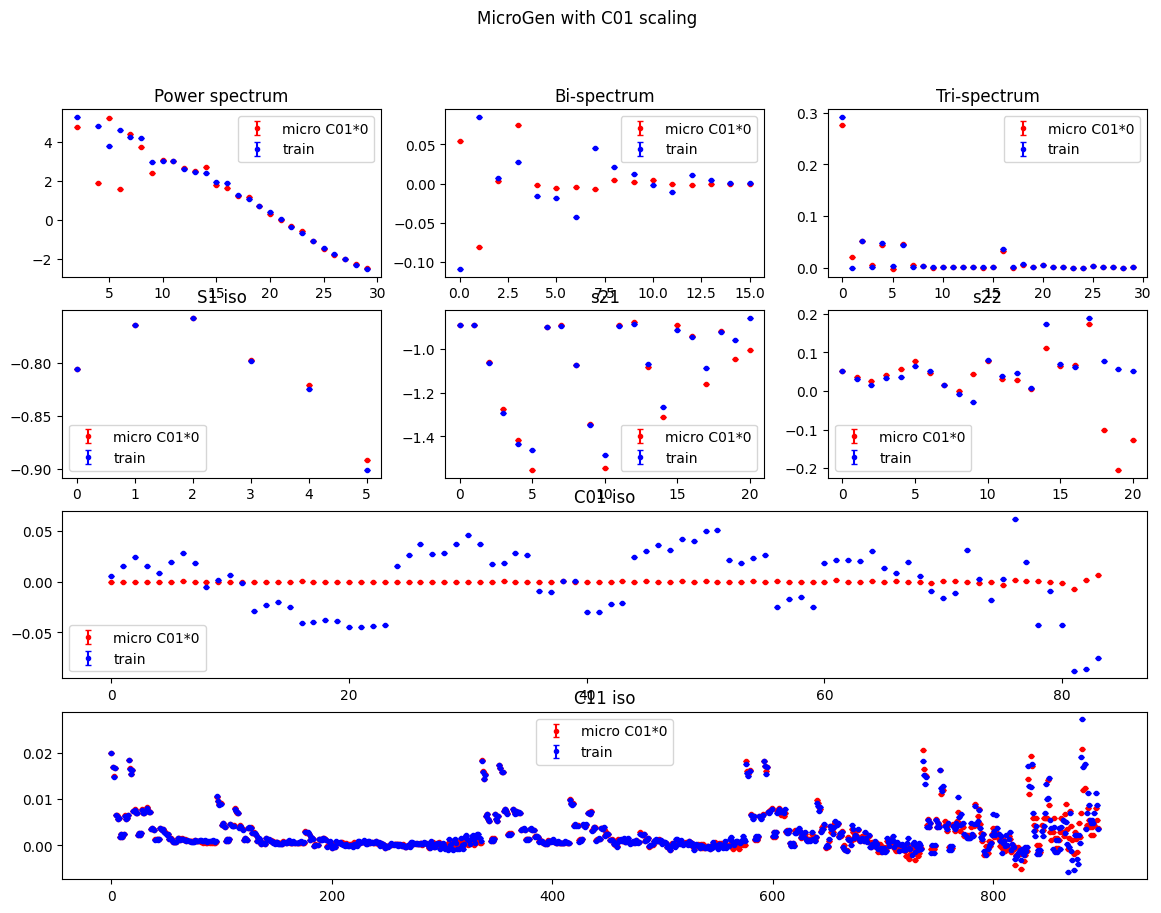
\includegraphics[width=0.99\textwidth]{fig-WL1-micro-C01scaling.png}
\caption{Statistiques de la figure \ref{fig-WL1-summary-stat} mais concernant les données WL-1 et un modèle micro-canonique du type de celui discuté à la section \ref{sec-WL1-res} mais où les coefficients $C_{01}$ sont volontairement mis à 0. Notons que l'on a utilisé qu'une unique carte pour calculer les distributions.}
\label{fig-WL1-micro-C01scaling}
\end{figure}
Au-delà de la distribution des $C_{01}^{iso}$, l'hypothèse d'une corrélation des désaccords $C_{01}^{iso}$,  bi-spectrum et $s_{21}$ peut sembler avoir un certain sens.
\end{itemize}
%
\section{Conclusion}
% 
Dans cette note, nous avons exposé les résultats de calculs de statistiques permettant d'aller au-delà de l'aspect visuel et spectre de puissance, afin d'apprécier la qualité des cartes générées par des modèles WCRG dans le cas de données de Weak Lensing et $\phi_4$. Ce qui en ressort à l'heure de l'écriture de cette note, c'est que si globalement les distributions d'ordre supérieur sont bien reproduites, ce qui est un résultat nouveau très encourageant, il en reste une qui fait défaut à savoir celle des coefficients de corrélations\footnote{Notons que nous n'avons pas montré les distributions les distributions des coefficients "non-iso" mais nous avons vérifié que  les désaccords sont identiques à ceux observés dans cette note.} $C_{01}$.  Sauf en fait dans un cas particulier, à savoir $\phi_4$ avec $\beta=0.50$, mais il se trouve que la distribution des $C_{01}$ obtenue sur les cartes d'entraînement est nulle.

Donc, il "reste" à comprendre comment on peut améliorer la modélisation des potentiels WCRG afin d'obtenir de meilleurs résultats. Notons qu'un réseau DGAN optimisé sur les données WL-1 donne des cartes dont les statistiques sont en parfait accord avec celles obtenues sur les données d'entraînement. Il en va de même avec des modèles micro-canoniques mais qui par nature sont optimisés de telles distributions.

%%%%%%%%%%
%\newpage
\appendix
\section{Plots de contrôle...}
Les histogrammes de cette section sont issues de la phase de synthèse du modèle WCRG entraîner sur les données WL-1 (Sec.~\ref{sec-wcrg-WL1-synt}).
\begin{figure}[h]
\centering
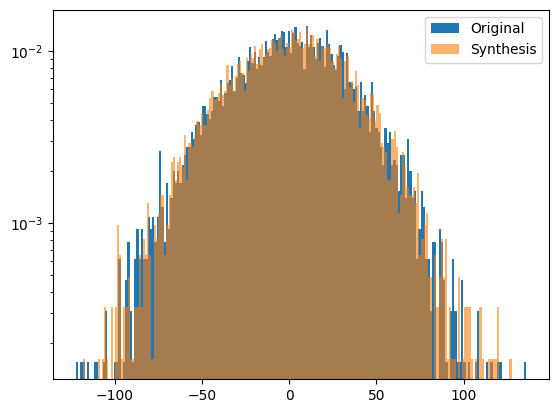
\includegraphics[width=0.35\textwidth]{fig-WL1-synt-L1-pixelval.png}
\caption{Comparaison des valeurs de pixels à l'échelle $L=1$.}
\label{fig-WL1-synt-L1-pixelval}
\end{figure}

\begin{figure}
\centering
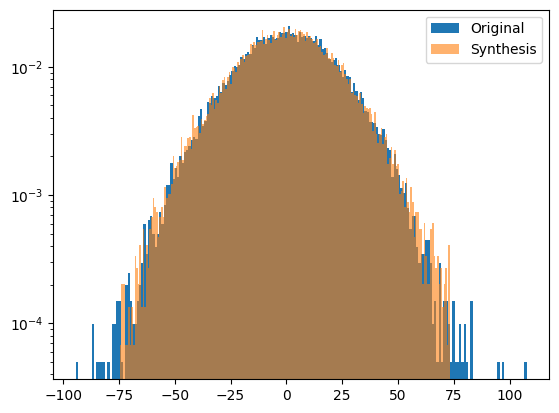
\includegraphics[width=0.35\textwidth]{fig-WL1-synt-L2-pixelval.png}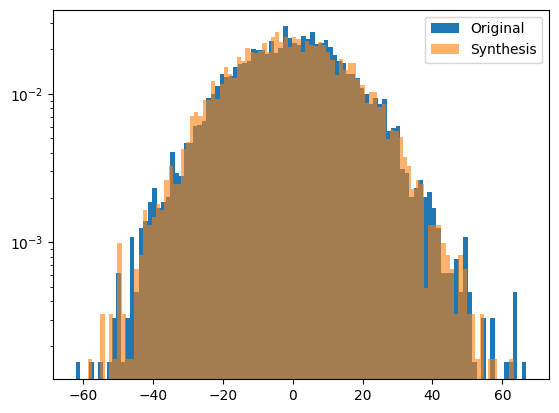
\includegraphics[width=0.35\textwidth]{fig-WL1-synt-L2-details_1.png}\\
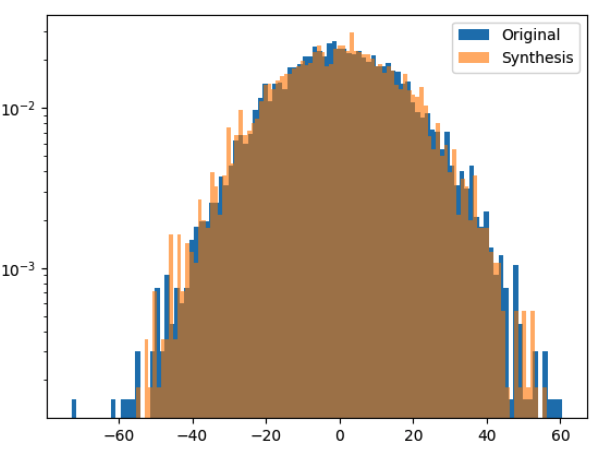
\includegraphics[width=0.35\textwidth]{fig-WL1-synt-L2-details_2.png}
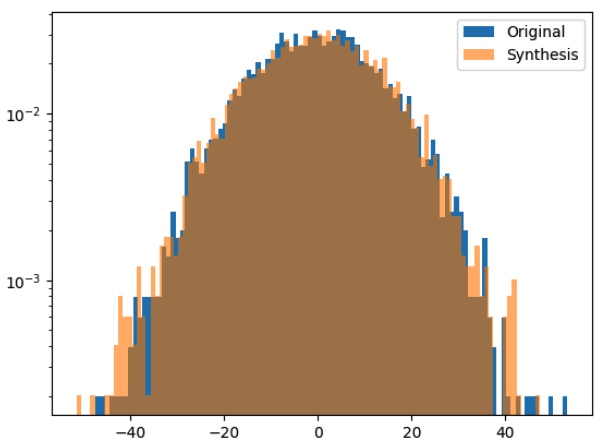
\includegraphics[width=0.35\textwidth]{fig-WL1-synt-L2-details_3.png}
\caption{Comparaison à l'échelle $L=2$ entre cartes de type "originale/entraînement" et de type "synthétisée": distribution des valeurs de pixels de cartes "totales" (haut-gauche), de détails "H" (haut-droite), de détails "V" (bas-gauche) et de détails "D" (bas-droite). }
\label{fig-WL1-synt-L2}
\end{figure}

\begin{figure}
\centering
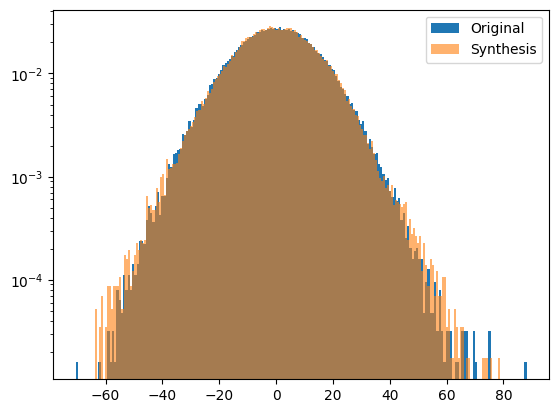
\includegraphics[width=0.35\textwidth]{fig-WL1-synt-L4-pixelval.png}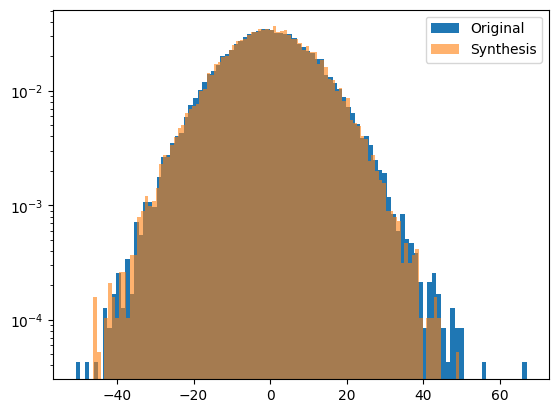
\includegraphics[width=0.35\textwidth]{fig-WL1-synt-L4-details_1.png}\\
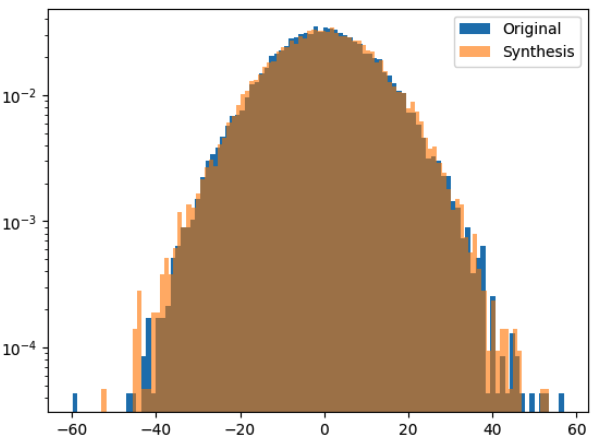
\includegraphics[width=0.35\textwidth]{fig-WL1-synt-L4-details_2.png}
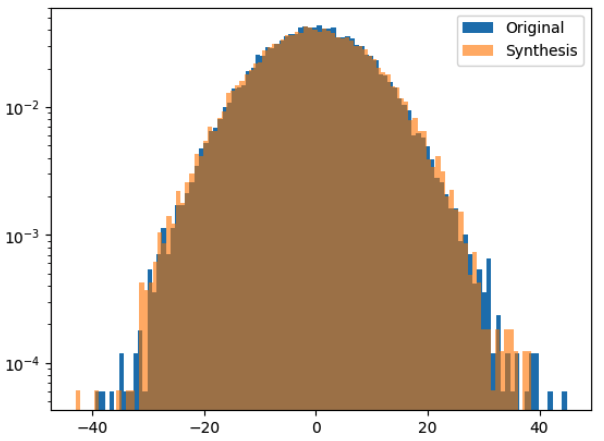
\includegraphics[width=0.35\textwidth]{fig-WL1-synt-L4-details_3.png}
\caption{Echelle $L=4$: légende identique à la figure \ref{fig-WL1-synt-L2}.}
\label{fig-WL1-synt-L4}
\end{figure}

\begin{figure}
\centering
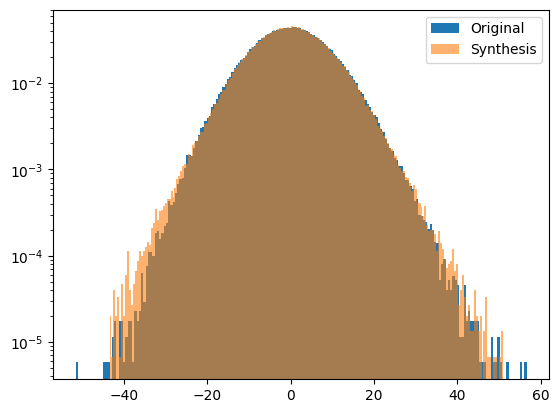
\includegraphics[width=0.35\textwidth]{fig-WL1-synt-L8-pixelval.png}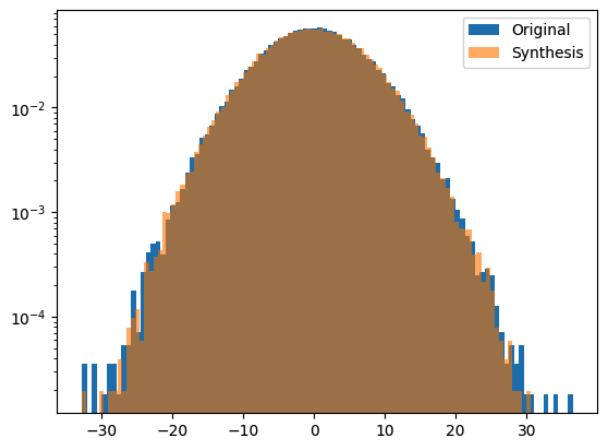
\includegraphics[width=0.35\textwidth]{fig-WL1-synt-L8-details_1.png}\\
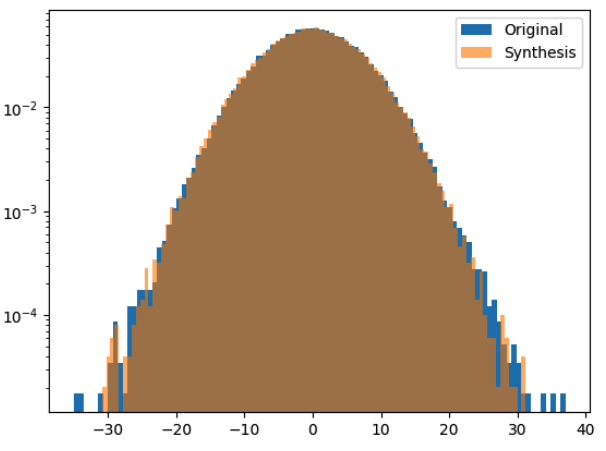
\includegraphics[width=0.35\textwidth]{fig-WL1-synt-L8-details_2.png}
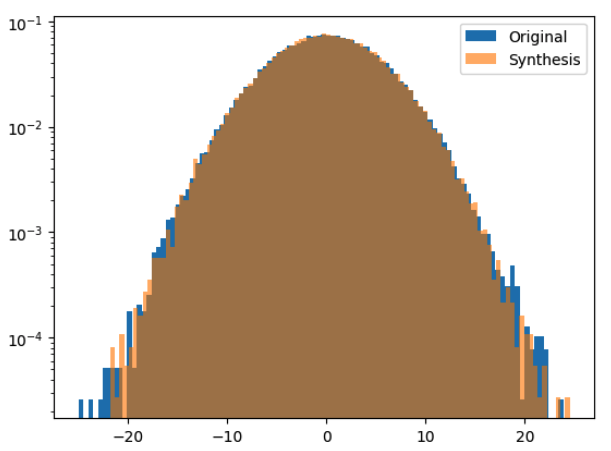
\includegraphics[width=0.35\textwidth]{fig-WL1-synt-L8-details_3.png}
\caption{Echelle $L=8$: légende identique à la figure \ref{fig-WL1-synt-L2}.}
\label{fig-WL1-synt-L8}
\end{figure}


\begin{figure}
\centering
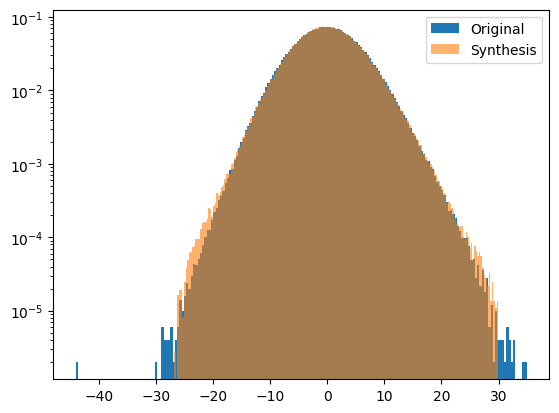
\includegraphics[width=0.35\textwidth]{fig-WL1-synt-L16-pixelval.png}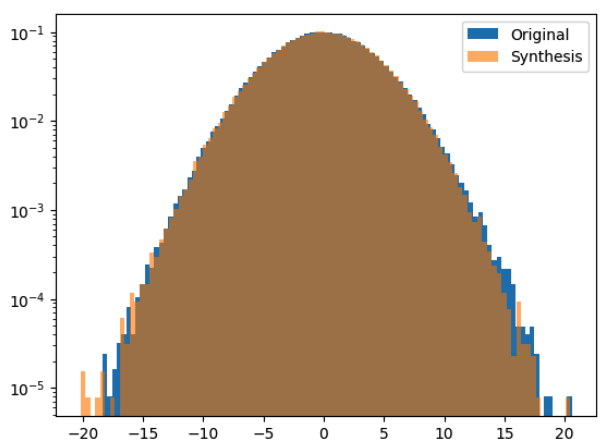
\includegraphics[width=0.35\textwidth]{fig-WL1-synt-L16-details_1.png}\\
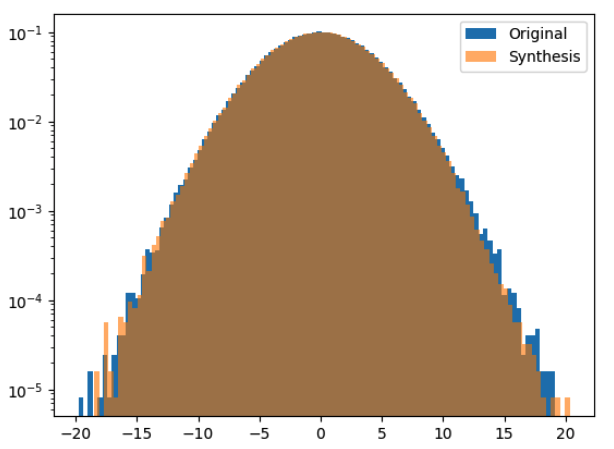
\includegraphics[width=0.35\textwidth]{fig-WL1-synt-L16-details_2.png}
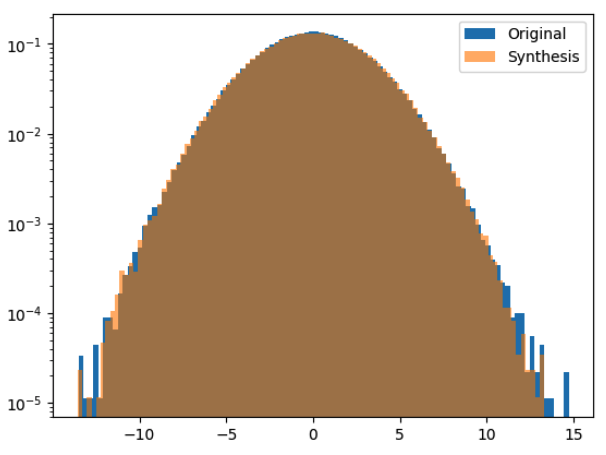
\includegraphics[width=0.35\textwidth]{fig-WL1-synt-L16-details_3.png}
\caption{Echelle $L=16$: légende identique à la figure \ref{fig-WL1-synt-L2}.}
\label{fig-WL1-synt-L16}
\end{figure}

\begin{figure}
\centering
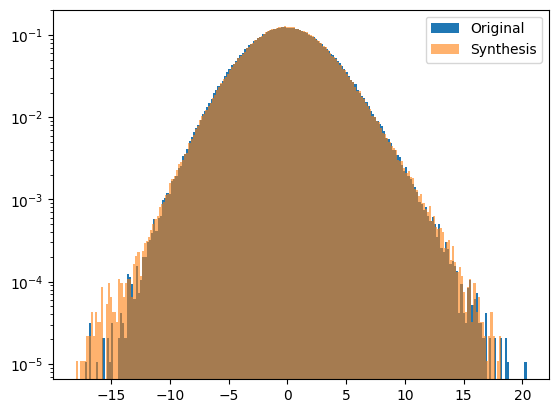
\includegraphics[width=0.35\textwidth]{fig-WL1-synt-L32-pixelval.png}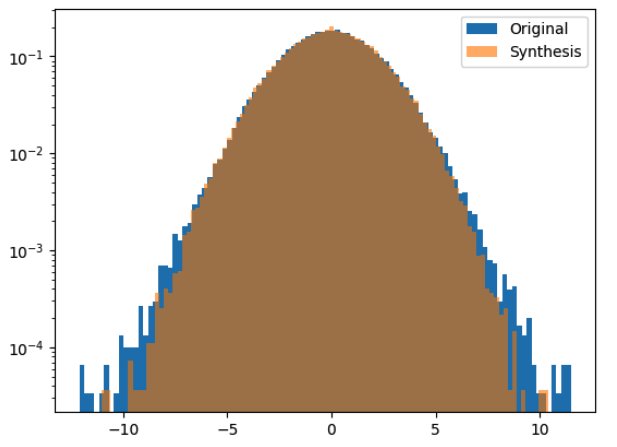
\includegraphics[width=0.35\textwidth]{fig-WL1-synt-L32-details_1.png}\\
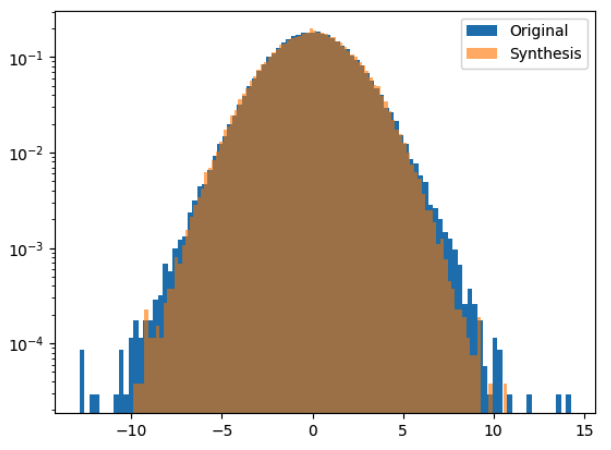
\includegraphics[width=0.35\textwidth]{fig-WL1-synt-L32-details_2.png}
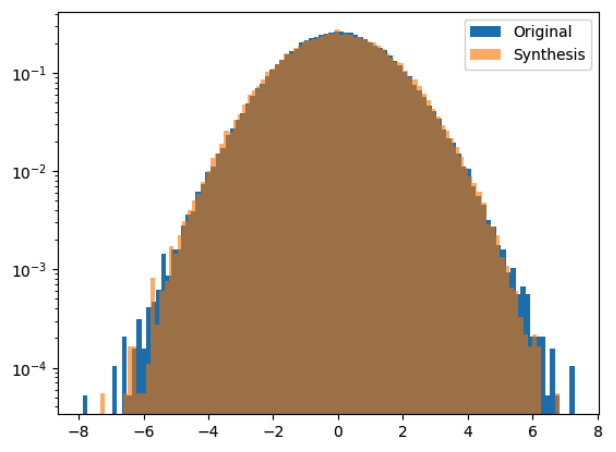
\includegraphics[width=0.35\textwidth]{fig-WL1-synt-L32-details_3.png}
\caption{Echelle $L=32$: légende identique à la figure \ref{fig-WL1-synt-L2}.}
\label{fig-WL1-synt-L32}
\end{figure}

\begin{figure}
\centering
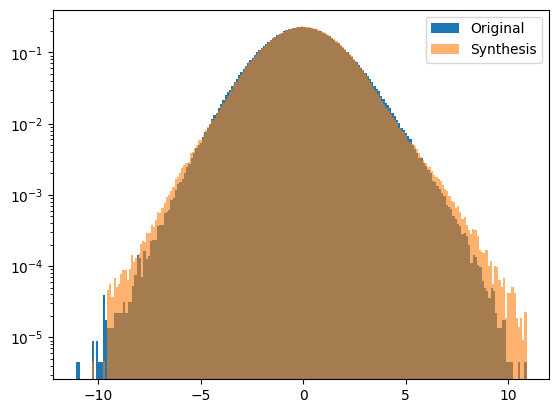
\includegraphics[width=0.35\textwidth]{fig-WL1-synt-L64-pixelval.png}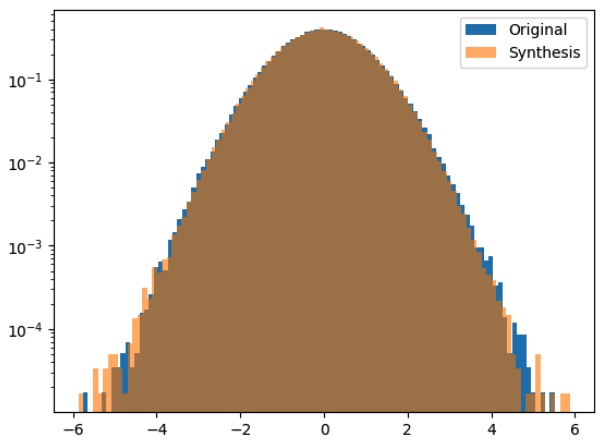
\includegraphics[width=0.35\textwidth]{fig-WL1-synt-L64-details_1.png}\\
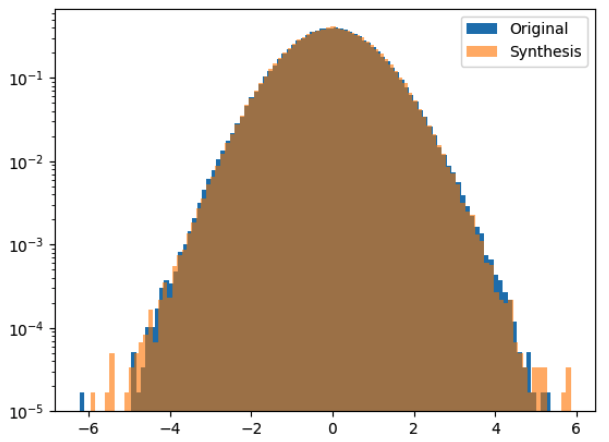
\includegraphics[width=0.35\textwidth]{fig-WL1-synt-L64-details_2.png}
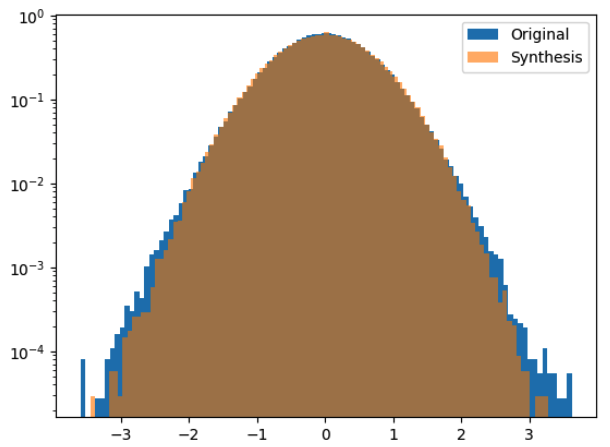
\includegraphics[width=0.35\textwidth]{fig-WL1-synt-L64-details_3.png}
\caption{Echelle $L=64$: légende identique à la figure \ref{fig-WL1-synt-L2}.}
\label{fig-WL1-synt-L64}
\end{figure}


\begin{figure}
\centering
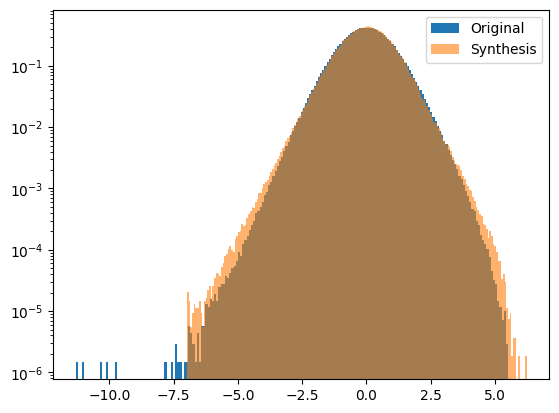
\includegraphics[width=0.35\textwidth]{fig-WL1-synt-L128-pixelval.png}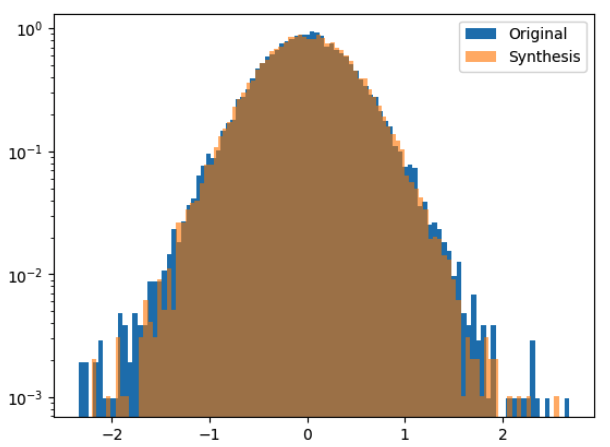
\includegraphics[width=0.35\textwidth]{fig-WL1-synt-L128-details_1.png}\\
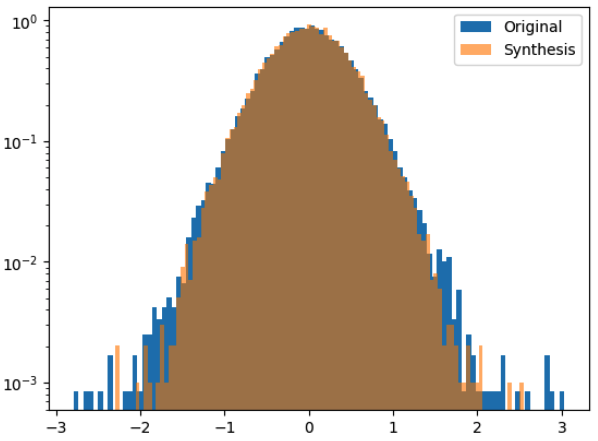
\includegraphics[width=0.35\textwidth]{fig-WL1-synt-L128-details_2.png}
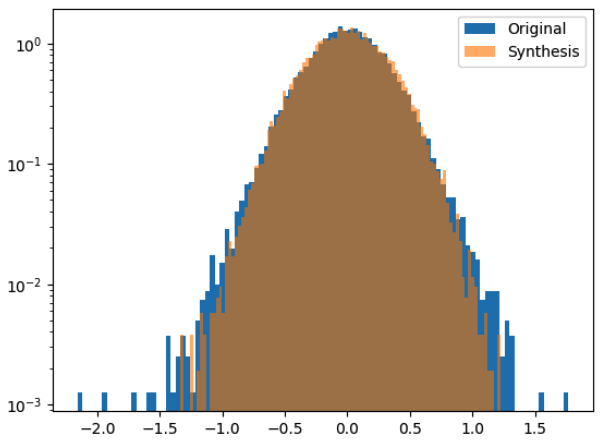
\includegraphics[width=0.35\textwidth]{fig-WL1-synt-L128-details_3.png}
\caption{Echelle $L=128$ (la plus grande possible): légende identique à la figure \ref{fig-WL1-synt-L2}.}
\label{fig-WL1-synt-L128}
\end{figure}

%%%%%%%%%%%%%%%%%%%%%%%%%%%%%%%%%
\newpage
\addcontentsline{toc}{section}{Références}
% Put your bibiliography file here
%\section{Bibliography}
\bibliographystyle{aa}
\bibliography{refs.bib}

\end{document}
